%%%%%%%%%%%%%%%%%% Environment
\documentclass[12pt]{article}
\usepackage[utf8]{inputenc}
%\documentclass{article}
%\usepackage{beamerarticle}

%%%%%%%%%%%%%%%%%% Basic Packages
\usepackage{amsbsy}
\usepackage{amstext}
\usepackage{amsfonts}
\usepackage{amssymb}
\usepackage{amsthm}
\usepackage{amsmath}
\usepackage{bbm}
\usepackage{color}
\usepackage{arydshln}
\usepackage{multirow}
\usepackage{changepage}
\usepackage{threeparttable,booktabs}
\usepackage{enumitem}
\usepackage{subfigure}
\usepackage{natbib}

%\usepackage{natbib}
%\bibliographystyle{abbrvnat}
%\setcitestyle{authoryear,open={((},close={))}}


%%%%%%%%%%%%%%%%%% Style
\usepackage[margin=1in]{geometry}%
\usepackage{setspace}
\doublespacing
%\usepackage{setspace}
%\setstretch{1.618}
%%%%%%%%%%%%%%%%%% Fonts and Graphics
\usepackage[cjk]{kotex} %Korean TeX
\usepackage[pdftex]{graphicx}

%%%%%%%%%%%%%%%%%% Theorem
\newtheorem{Theorem}{Theorem}
\newtheorem{Lemma}{Lemma}
\newtheorem{assumption}{Assumption}
\newtheorem{prop}{Proposition}
\newtheorem{corollary}{Corollary}
\newcommand{\ju}{\textcolor{cyan}}
\newcommand{\yj}{\textcolor{magenta}}
\usepackage{apptools}
\AtAppendix{\counterwithin{Lemma}{section}}
\AtAppendix{\counterwithin{table}{section}}
\AtAppendix{\counterwithin{figure}{section}}

%%%%%%%%%%%%%%%%%% Bibliography and Appendices
%\usepackage[natbibapa]{apacite} % Including URLs in bibliography
\usepackage{natbib}
\usepackage[hyphens]{url} % Including URLs in bibliography
%\usepackage[toc,page,title]{appendix} % Extra control of appendices
\usepackage[titletoc,toc,title]{appendix}
\usepackage{chngcntr}

%%%%%%%%%%%%%%%%%Appendix title
\let\oldappendix\appendix
\makeatletter
\renewcommand{\appendix}{%
  \addtocontents{toc}{\let\protect\numberline\protect\appendixnumberline}%
  \renewcommand{\@seccntformat}[1]{Appendix~\csname the##1\endcsname\quad}%
  \oldappendix
}
\makeatother

%%%%%%%%%%%%%%%%%% Beginning of the Manuscript
\begin{document}

\begin{center}{\LARGE Sharing Economy in the Cloud:}\end{center}
\begin{center}{\LARGE Pricing Schemes for Peer-to-Peer Storage Platforms}\end{center}
%\maketitle
%
%
\begin{abstract}
	%\onehalfspacing
    %\setlength{\baselineskip}{15pt}
	\noindent
	{\normalsize
	% 2024-02-23 version (187 words)
	Encountering the unprecedented surge in data storage demands, peer-to-peer (P2P) storage platforms with blockchain technology have emerged as a viable alternative to conventional cloud storage services. While crowdsourcing unused storage resources in P2P storage platforms might be securely conducted with blockchain, the decentralized structure does not ensure sufficient storage availability. This paper examines incentive schemes to encourage user participation in the platform for storage capacity and access: the two-part tariff, the subscription, and the hybrid pricing. Using a game-theoretic approach, we consider a profit-seeking platform by incorporating interplays among renters and providers and the platform's algorithmic decision under a given pricing scheme. We show that the two-part tariff maximizes short-run profits for the platform and providers, while subscription-based pricing shows the highest renter surplus. Considering all stakeholders, we find that the optimal pricing scheme differs by the size of potential providers. When there are enough providers to meet the storage demand from renters, the overall welfare is higher with the subscription-based pricing that maximizes renters' welfare. However, we show that the hybrid pricing or the two-part tariff maximizes social welfare when potential service providers are relatively scarce.}
\end{abstract}
%\baselineskip 15.5pt
\hspace{0.2cm} {\sc Keywords:} Cloud computing; peer-to-peer markets; pricing schemes; sharing economy
%
%
\clearpage
%
%
\begin{center}\textbf{\large INTRODUCTION}\end{center}

\noindent Despite the rapid growth of public cloud services such as Amazon Web Services (AWS), the supply of the storage capacity is expected to be insufficient to meet the unprecedented demands of data volume in the near future. According to the International Data Corporation (IDC), the global spare storage capacity ratio in a commercial market is expected to be reduced from 33 percent in 2018 to 15 percent in 2020 \citep{robb2015space, idc2018worldwide}. As a prompt remedy for this upcoming shortage problem, a plausible solution can be the efficient use of available storage space scattered over billions of personal computers (PCs). The total non-commercial hard drive space on PCs is estimated to be nearly 250 exabytes (or 250,000 petabytes) globally, which is larger than the capacity of all public cloud services combined \citep{thompson2014cloud}.\footnote{In 2012, Facebook stored 100 petabytes (PB), Microsoft stored 300 PB, and Amazon held 900 PB of data in its S3 cloud service.} If individual users can successfully share their under-utilized hard-drive spaces with potential renters, this can be a valuable complementary and competing service against conventional public cloud services. However, data storage sharing between PCs as a direct form of peer-to-peer (P2P) transactions has not been widely implemented for several notable reasons, such as information privacy and security concerns.

To adequately deal with these non-negligible issues, new data storage and sharing platforms integrating various Industry 4.0 technologies such as cloud computing and blockchain have been emerging \citep{protocol2017filecoin, vorick2014sia, wilkinson2016storj}. The blockchain-enabled decentralized P2P storage platforms make under-utilized hard-drive spaces available for data storage services with advanced encryption technology. Specifically, the P2P file-sharing protocol allows renters to store large files in fragmented pieces distributed to many individual providers. In this way, no single provider has enough fragments to reconstruct the original file. Also, the original files can be reassembled only by a renter’s private key, further ensuring that storage providers cannot read the content. In addition, the platforms use novel blockchain technology, by which storage contracts between renters and providers are recorded and verified collaboratively. Peers are incentivized or penalized based on their contributions to the network, leading to a stable resilience of the system.

While P2P storage services are still beginning, they have already attracted significant attention in the cryptocurrency market with massive successes from the initial coin offerings (ICOs). For instance, Storj, a platform that appeared in 2014, has already reached a market capitalization of \$391.0 million with a total storage capacity of 36.7 PB, 71,689 platform users, and 285 million files. Similarly, Sia has reached a market capitalization of \$872.9 million. It has a total 3.5PB storage capacity and 1.2 million accumulated downloads. Filecoin, which appeared relatively recently, set a new record in ICO funding of \$257 million in 2017 and currently ranks 24th among all cryptocurrencies with a market capitalization of \$6.816 billion. Surprisingly, it reached a total 629.3PB storage capacity within ten months from its service launch. These cases demonstrate the expectation that P2P file-sharing services will rapidly grow by successfully mitigating security issues with a blockchain-enabled decentralized approach.\footnote{Please refer to recent statistics of Storj, Sia, and Filecoin from https://www.storj.io/, https://siastats.info/, and https://file.app/, respectively. All statistics in this paragraph were observed on August 12, 2021.} Also, at the same time, it raises a question to attract and secure a greater number of participants to transit to the next stage.

In fact, the decentralization creates an undesirable problem regarding storage availability. P2P platforms are not in control of the storage capacity and online connection to the stored files, so it is not easy to maintain and control agreeable service levels on both of them. In this regard, the P2P storage platforms rely mainly on various economic incentives to attract and maintain providers to ensure a sufficient level of storage availability in terms of the storage capacity and the online connection to the storage \citep{babich2020distributed, beck2018governance}. The P2P platforms currently charge renters two parts of fees: a storage service fee for providers sharing the storage space with renters and a bandwidth service fee for maintaining providers' online connection to the shared storage for renters. Sia, for example, has used a two-part tariff that imposes a base storage fee for using the storage capacity and a bandwidth fee for each download request to stored data. Similarly, Storj had charged the same type of fees for both services. Recently, Storj has introduced a new pricing scheme that provides free usage volume up to a certain threshold.\footnote{Storj's latest pricing policy is available at https://www.storj.io/pricing.} Once renters' download requests exceed this point, the platform starts imposing the bandwidth service fee. Although these platforms need to carefully design their pricing schemes to gather potential providers and renters effectively, little is known about the impact of possible pricing schemes on providers, renters, and the platform for this new and immature market. 

Thus motivated, this study aims to investigate a P2P storage platform's optimal design of service fees, storage redundancy algorithms, and the implications of pricing schemes on profit and surplus. We incorporate pricing schemes that either centralized public cloud services or P2P storage platforms have adopted in practice. Specifically, P2P storage platforms have widely adopted the two-part tariff, while conventional public cloud services have widely used the pay-per-use, subscription-based, and hybrid pricing \citep{kansal2014pricing}. We compare the effectiveness of these pricing schemes and their impacts on services, e.g., whether a specific pricing scheme that burdens renters for the provider's operating costs indeed brings benefits to the platform and whether the subscription-based scheme is appropriate for the decentralized P2P storage services.

Specifically, we consider three pricing schemes: First, we investigate the two-part tariff (a lump-sum fee for the storage capacity + pay-per-use fee for the download bandwidth). Second, we incorporate the subscription-based pricing, where renters gain unlimited free access to stored files after paying for the storage capacity. Finally, we consider the hybrid pricing, which provides a lump-sum fee for the storage and a limited allowance of free bandwidth service that charges a pay-per-use fee for excess downloads. Regarding these pricing schemes, we intend to analyze their consequences on P2P storage services by answering the following research questions:
\begin{itemize}
    \item How should the platform decide its redundancy algorithm and service fees according to the pricing scheme?
    \item Which pricing scheme would maximize the platform's profit/the overall system surplus?
    \item How do the numbers of potential renters and providers in the two-sided market affect the effectiveness of pricing schemes?
\end{itemize}

To answer these questions, we build a game-theoretic model of a profit-seeking P2P storage platform that intermediates storage providers and renters. In our model, the P2P storage platform sets its redundancy algorithm and service fees within the given pricing scheme. Then, storage providers with heterogeneous operational costs decide whether to join this P2P storage platform and share their unused storage capacity with renters. Finally, storage renters with heterogeneous willingness to pay for the storage service determine whether to adopt the P2P storage platform. For completed transactions between providers and renters, the platform charges commission rates to make a profit. We assume that the operating cost incurred by a storage provider increases with a bandwidth usage level that varies across renters. In storing a renter's file, the platform uses a redundancy algorithm (a $k$-of-$m$ erasure coding scheme) that divides each file into $k$ fragments and assigns encrypted copies of these fragments to $m$ ($> k$) providers. Here, we define the redundancy rate as the stored volume divided by the original file volume, $m/k$. Thus, the platform can only satisfy storage demand up to participating providers' capacity, divided by the redundancy rate. Based on this model setting, we analyze the platform's choice of service fees under each pricing scheme and compare the platform's profit and the system surplus across the pricing schemes.

Our results suggest that the platform should set the redundancy algorithms minimizing the total providers' operating costs for all pricing schemes. We also show that when the first-best prices---which maximizes the platform's profit when the size of potential providers is sufficient---are applicable, the two-part tariff always maximizes the platform's profit and provider surplus, and the hybrid pricing follows. Notably, we see that the hybrid pricing yields the same outcomes when it offers a small amount of free-download volume. Regarding the renter surplus, the subscription-based pricing is most effective because the gain of renters with a higher usage frequency exceeds the loss from renters leaving the service due to a high storage fee. Consequently, the subscription-based pricing outperforms other pricing schemes regarding the total surplus.

Markedly, we find that the impacts of pricing schemes significantly differ when potential providers are relatively scarce. If the size of potential providers is insufficient to fulfill the storage demand, the platform's optimal fees are subject to the market-clearing prices---which makes supply and demand equivalent---instead of the first-best prices. In this situation, the subscription-based pricing does not necessarily generate the maximum total surplus. In other words, the two-part tariff and the hybrid pricing can dominate the subscription-based pricing concerning the platform's profit and the total surplus. 

We further validate our findings by examining how endogenous commission rates affect the results. We find that our main insights continue to hold when the platform determines commission rates endogenously, although the thresholds that enable the first-best prices change accordingly. Moreover, we conduct numerical analyses with relaxing assumptions on renter heterogeneity and observe consistent results.

\begin{center}\textbf{\large RELATED LITERATURE}\end{center}

\begin{center}\textbf{\large Pricing and Capacity Management in Centralized Cloud}\end{center}

\noindent A rich body of literature has examined pricing schemes in centralized services. For instance, Randhawa and Kumar (2008) examined a rental firm that considers either a subscription option with the restricted number of simultaneous rentals or a pay-per-use option without such restriction. They showed that the subscription option yields higher social welfare and consumer surplus. Cachon and Feldman (2011) studied a queueing model that compares subscription and pay-per-use schemes where congestion incurs disutility. They found that subscription pricing is more profitable than pay-per-use pricing particularly if customers are more heterogeneous in their service rates.

Recently, there has been growing interest in studying pricing strategies and capacity management for centralized cloud platforms \citep{fazli2018effects, chen2019pricing, chen2021discount, li2018should, kansal2014pricing, arbabian2021capacity}. For instance, \citet{chen2019pricing} considered two pricing schemes in cloud platforms: the reservation-based scheme and the utilization-based scheme. The former ensures a certain number of instances during the contract term (similar to the subscription-based pricing), while the latter charges customers based on the realized demand (similar to the pay-per-use). Considering a duopoly model where cloud platforms adopting different schemes compete for customers with heterogeneous usage, they found that customers with lower demand volatility would prefer the reservation-based scheme, whereas those with higher volatility would prefer the utilization-based scheme.

\citet{nunez2021leveraging} proposed pricing schemes for Infrastructure as a Service (IaaS) cloud services, aiming to manage slack capacity and low utilization of resources. They combined two types of served-instance (contract) and on-demand services and examined their effectiveness across different market conditions in terms of service rate, market size, and service reliability. \citet{fazli2018effects} examined how autoscaling, which allows firms to scale their computational load to match customer demand automatically, affects market entry decisions, equilibrium prices, profitability, and consumer surplus. They showed that autoscaling might alleviate price competition because it reduces uncertainty about demand and excessive computational capacities.

These studies have mainly focused on pricing schemes and their role in managing capacity in centralized cloud platforms. Despite the advances in this research stream, little research has examined the role of pricing schemes in capacity management in P2P cloud platforms. Considering that P2P services hinge upon independent providers, pricing decisions affect not only service demand and utilization but also the supply level of providers. Thus, neglecting this two-sided aspect inhibits us substantially from understanding the impact of pricing schemes on P2P cloud platforms.

\begin{center}\textbf{\large P2P Sharing of Computing Resources}\end{center}

\noindent This paper is also related to the literature on sharing platforms for computing resources. The vast majority of studies in this stream focused on the mechanism design of P2P file-sharing networks \citep{antoniadis2004p2p, casadesus2010p2p, de2017quality, ghasemkhani2018contracting, golle2001incentives}. For instance, \citet{antoniadis2004p2p} conducted a numerical analysis to compare several incentive schemes and suggested that a simple fixed fee scheme, where all peers are required to share a standard number of files, can achieve a high level of network efficiency. \citet{de2017quality} studied how individual peers make sharing decisions under quality-of-service based pricing schemes. They showed that socially optimal behaviors are induced where a pricing scheme does not charge users for content requests, while profit maximization is achieved where a pricing scheme charges users for requesting content. \citet{ghasemkhani2018contracting} proposed a contracting scheme for a monopolistic P2P file-sharing network, in which the network compensates each contracted peer node for the supply of files. They investigated the optimal reward scheme for the profit-seeking P2P network regarding network structures, content availability, propagation delay, among others.

It is worth noting that this literature stream has concentrated on file-sharing platforms only. Although a variety of computing resources---such as storage capacity, CPU power, and internet bandwidth---have recently been shared in online markets \citep{dickson2019monetizing, sharma2020blockchain}, we are aware of no study that examined sharing platforms for these resources.

\begin{center}\textbf{\large Sharing Economy and Online Platforms}\end{center}

\noindent Several studies examined the benefit of sharing idle resources through these platforms. For example, \citet{zervas2017rise} provided empirical evidence that Airbnb's entry lowered hotel prices which are beneficial for consumers. \citet{lee2018battle} demonstrated that Uber significantly reduces search costs for riders. While numerous studies echoed that emerging sharing platforms are good for consumers \citep{einav2016peer, greenwood2017show}, some analytic studies indicated that those platforms are not necessarily beneficial to consumers in the long term as they might increase product prices or discriminate consumers \citep{abhishek2021business, jiang2018collaborative, weber2016product}. \citet{tian2018effects} showed that a sharing platform tends to increase the retailer's share of the gross profit margin in the distribution channel.

Recent studies have suggested theoretical frameworks for pricing strategies in sharing platforms \citep{bai2019coordinating, benjaafar2019peer, cachon2017role, bimpikis2019spatial, taylor2018demand}. \citet{benjaafar2019peer} considered both profit-maximizing and social-welfare-maximizing platforms and compared their equilibrium outcomes. They found that the differences in the social welfare between these platforms are relatively modest. \citet{cachon2017role} examined several pricing schemes, including the surge pricing, for sharing platforms with self-scheduling providers. They found that the surge pricing generally achieves nearly the optimal profit and improves the surplus of providers and consumers as labor becomes expensive. Recently, \citet{zhang2022two} studied the effects of wage schemes, such as fixed commission rate, dynamic commission rate, and fixed wage, on competition between sharing platforms. They showed that the relative competitiveness between the supply and demand sides determines which wage scheme is more effective in facilitating the profits for platforms and surpluses for consumers and workers.

\begin{center}\textbf{\large Contributions to the Literature}\end{center}

\noindent Our study is the first attempt to provide a theoretical framework for pricing in decentralized cloud platforms. Unlike centralized cloud services, P2P cloud platforms do not have direct control over service capacities and rely on independent providers with unused storage capacity. Therefore, their pricing decisions affect both customers' costs and service levels. We develop a model that accounts for this complexity by incorporating providers' service participating decisions, renters' service adoption decisions, and the interactions between providers and renters.

Furthermore, we investigate the potential of the pricing scheme that P2P storage platforms have not explicitly implemented yet---the subscription-based pricing, which has been widely adopted in conventional public cloud services \citep{kansal2014pricing}. We show that the impacts of pricing schemes on the system surplus can change by the relative number of potential providers compared to the storage demand from renters. When there are a sufficient number of potential providers, the subscription-based pricing, which P2P storage platforms have neglected in practice, always produces the highest renter surplus and the highest system surplus. Interestingly, the two-part tariff or the hybrid pricing can dominate the subscription-based pricing regarding the platform's profit and the total surplus when the number of potential suppliers is insufficient to satisfy the storage demand.

In addition, we incorporate the platform's algorithmic decision into our framework by considering peer decisions in the supply and demand sides. We show that P2P platforms need to set the redundancy algorithm to minimize the total operating costs of providers in the system, and interestingly, this algorithmic decision is independent of pricing schemes. These findings suggest that P2P storage platforms can improve their pricing strategies and redundancy algorithms separately, even though each decision affects providers and renters simultaneously.

Our study also extends the literature on P2P sharing of computing resources. Recently, emerging platforms have enabled sharing of various computing resources, such as storage capacity, CPU power, and internet bandwidth \citep{dickson2019monetizing, sharma2020blockchain}. However, no study has contributed to our understanding of sharing platforms for these resources. Unlike P2P file-sharing services, P2P storage sharing comprises the initial storage service and the subsequent bandwidth service. Thus, a two-part tariff consisting of a lump-sum charge (storage fee) and a per-unit charge (bandwidth fee) is widely adopted in practice. Hence, the existing framework for file-sharing platforms, where consumers are satisfied once they receive appropriate files, cannot be directly applied. We expect that our framework for P2P cloud storage, which prior studies have not examined, can provide valuable insights for sharing services of various computing resources. 

Lastly, this study contributes to the literature on the pricing for sharing economy in general. We show that pricing schemes that reward providers can improve the system surplus when the potential suppliers are too scarce compared to consumers. In this situation, the impact of pricing schemes varies according to the degree of scarcity of suppliers. For instance, P2P delivery platforms that serve various regions in terms of the number of sellers, deliverers, and consumers might offer different pricing schemes across regions according to the relative scarcity of sellers or deliverers compared to consumers to improve the surplus of overall stakeholders. Prior studies on pricing in the sharing economy, such as \citet{cachon2017role} and \citet{zhang2022two}, did not consider the potential of the pricing schemes that we have examined in this paper. Specifically, these studies postulated a common price and focused on the price-wage relationships---i.e., how the platform should share its revenue with workers---rather than on how to price services depending on usage levels. Consequently, these studies paid scant attention to comparing service pricing schemes, such as the two-part tariff, subscription-based pricing, and hybrid pricing In fact, the two-part tariff that consists of lump-sum fees and pay-per-use can also be used in other sharing platforms (e.g., base rates and cost-per-user in ride-sharing platforms). Hence, our model can extend these studies by enhancing insights on sharing platforms' pricing strategies.

Also, unlike \citet{cachon2017role}, we allow providers to have heterogeneous operating costs, which are also affected by renters' usage levels. Specifically, we postulate that individual providers have different sensitivities to their uptime level and a higher usage level of a renter leads to a higher operating cost of a provider, which is not the typical model setting in the sharing economy literature. By incorporating this cost structure, we can examine the impact of providers' in-out decisions and the operational burden of bandwidth services.\\

\begin{center}\textbf{\large MODEL}\end{center}

\noindent In this section, we first describe our model setups and players, which is followed by the key decisions of players. We present the summary of basic notations in Table \ref{tbl:summary}.

\begin{table}[h] \centering
\textbf{\caption{A Summary of Basic Notations}\label{tbl:summary}}
\vspace{0.1in}
\begin{tabular}{l  p{14cm}}
\toprule
\textbf{Notation} & \textbf{Description} \\\hline
\multicolumn{2}{l}{\textbf{Parameters: Environment}}\\\hline
$n_r$ & Number of potential renters \\
$n_p$ & Number of potential providers \\
$\alpha$ & Proportion of revenue that providers receive \\\hline
\multicolumn{2}{l}{\textbf{Parameters: Heterogeneity}}\\\hline
$u_i$ & Renter $i$'s unit utility of bandwidth usage \\
$\lambda_i$ & Renter $i$'s bandwidth usage \\
$\rho_j$ & Provider $j$'s sensitivity to bandwidth provision\\\hline
\multicolumn{2}{l}{\textbf{Platform's decision variables}}\\\hline
$\theta$ & (Algorithm decision) Redundancy rate \\
$t$ & (Algorithm decision) Required uptime, determining unit operating cost $\xi$\\
$p_s$ & (Pricing decision) Storage fee\\
$p_b$ & (Pricing decision) Bandwidth fee\\\hline
\multicolumn{2}{l}{\textbf{Performance measures}}\\\hline
$\Pi$ & Platform's profit\\
TS & Total system surplus\\
\bottomrule
\end{tabular}
\end{table}

\begin{center}\textbf{\large Model Setups}\end{center}

\noindent We consider a P2P storage platform where some peers provide their unused storage (hereafter, \textit{providers}) and other peers rent the storage space and request downloading of stored files (hereafter, \textit{renters}). The platform offers two services to renters: \textit{i)} the initial file storage (the storage service), and \textit{ii)} access to the stored files via a download request (the bandwidth service). Once a renter requests storage space to save a file, a platform divides her file into $k$ fragments and assigns them to $m$ ($> k$) providers.\footnote{P2P storage platforms employ a $k$-of-$m$ erasure coding scheme, under which an original file is divided into $k$ shards, and the shards are re-coded into $m$ encrypted fragments ($m > k$) \citep{wilkinson2016storj}. Since any $k$ fragments among $m$ fragments are sufficient to reconstruct the file, erasure coding enables high reliability with low expansion factors \citep{weatherspoon2002erasure}.} After completing the initial file storage, a renter can request a download of the stored file to the providers.

Since the availability of stored files to storage renters is critical for P2P storage services, the P2P storage platforms should maintain the likelihood of file transfer failure negligible. Therefore, the platform needs to carefully set the algorithmic parameters: 1) the redundancy in the erasure coding $\theta \equiv \frac{m}{k}$, which refers to the proportion of the size of the duplicated data compared to the size of the original data, and 2) uptime $t$, which represents the proportion of provider's time being connected to the P2P network \citep{protocol2017filecoin, vorick2014sia, wilkinson2016storj}. We postulate that the platform considers the algorithm parameter combinations that maintain the same failure probability. In doing so, the platform may increase $\theta$ and decrease $t$ or vice versa. When the platform decides to raise $\theta$ and correspondingly reduce $t$, participating renters have to pay higher storage costs due to the higher redundancy rate, while providers can mitigate their operating burden. Consequently, the P2P network imposes a higher burden on renters. On the other hand, when the platform meets the probability by increasing $t$ rather than $\theta$, providers have to bear higher operating costs due to higher bandwidth uptime.

P2P storage platforms attempt to develop redundancy algorithms that ensure extremely low failure probabilities. Theoretically and practically, it has shown to be extremely rare for well-performing P2P networks to experience file transfer failure in practice.\footnote{For instance, the failure probability of a $k$-of-$m$ erasure coding is 5.266e-10 where $k=6$, $m=18$, and $t=0.90$ \citep{wilkinson2016storj}. In Sia's storage network, providers must maintain a 95–98\% uptime, enabling the network to achieve 99.9999\% availability of stored files to renters.} Thus, we assume that the P2P storage platform sets an availability goal that is sufficiently large and close to its upper bound, one, and only considers the $(\theta, t)$ combinations that satisfy this availability goal. As such, our model does not take the failure probability of the file transfer into account.

\begin{figure}[ht!]
\centering
\includegraphics[width=14cm]{fig1_timeline_minor_revision.pdf} 
\textbf{\caption{The Sequence of Events}\label{fig:timeline}}
\end{figure}

Figure \ref{fig:timeline} illustrates the sequence of the events for the platform, providers, and renters in our model. Specifically, the platform observes the potential market size of peers ($n_r$ and $n_p$). In response to the \textit{exogenously} given market condition, pricing scheme, and commission rate, the platform first determines its redundancy algorithm ($\theta$, $t$). Then, the platform decides its service fees $(p_s, p_b)$, which is consistent with the current market situation, where the development of a redundancy algorithm takes several months or years.\footnote{Sia and Storj have not officially changed their algorithms since their releases. Also, Sia has not adopted the 64-of-96 algorithm, which this platform announced its development plan in 2020. The announcement is available at https://blog.sia.tech/cloud-storage-for-2-tb-mo-8a34043e93bb.} After that, potential providers for this P2P storage service decide whether or not to join the platform based on their expected profits. Once a provider joins the platform, he provides unused storage spaces to renters. Lastly, observing the service fees and the available storage capacity, potential renters of the P2P storage service evaluate the expected utility and decide whether to adopt the service. Once adopting the P2P storage service, a renter starts using the storage spaces from providers.

We now further explain three essential players in the P2P file-sharing service: renters, providers, and a service platform.

\textbf{\textit{Renters.}} We consider a renter that needs a storage space for her unit volume of files. We denote the total number of potential renters in the market by $n_r$. Each potential renter decides whether to adopt the P2P storage platform and rent the storage space from providers. If a renter adopts the platform, she will obtain the usage value and pay the storage service fees for storing files to the providers' spaces and the bandwidth service fees for requesting a download of stored files. The renters will join the platform if their usage value exceeds the total service costs.

This model concerns renters with a continuum of bandwidth usage level (or frequency of download requests) of stored files denoted by $\lambda$. It has been empirically observed in the literature that the usage of cloud-resource is distributed with relatively heavy tails compared with exponential, log-normal, and normal distributions \citep{loboz2012cloud}, similarly to other digital resources like smartphone and YouTube usage \citep{falaki2010div, gill2008char}. Thus, we assume that a renter's bandwidth usage $\lambda$ follows the Pareto distribution in keeping with the extant literature \citep{bandi2015robust, li2018should, ramirez2017adapt}.

Based on this assumption, the probability distribution function of the bandwidth usage level can be expressed as $f(\lambda) = \frac{b \lambda_0^b}{\lambda^{b+1}}$, where the minimum bandwidth usage level is denoted by $\lambda_0$. For analytical tractability, we simplify our assumption such that the distribution of bandwidth usage level is characterized by the parameter value of $b = 2$. We also incorporate heterogeneous valuation of a renter's service usage. Specifically, we assume that renter $i$'s utility per unit volume of bandwidth usage (i.e., $u_i$) follows a uniform distribution; that is, $u_i \sim U[0, 1]$. As a result, renter $i$'s total utility obtained from storing files is $\lambda_i u_i$. To focus on the interplay among the platform, providers, and renters, we assume that $\lambda_i$ and $u_i$ are independent.

Renters pay the total service cost $c(p_s, p_b, \lambda_i)$ for their storage and bandwidth services according to the service fees ($p_s, p_b$) set by the P2P storage platform. This cost may change by $\lambda$ depending on a pricing scheme. As the utility per bandwidth volume $u_i$ is assumed to be bounded above and below by $0$ and $1$, the bandwidth service fee $p_b > 1$ will lead to a negative utility from the bandwidth for every renter. Thus, we restrict our attention to the case where the platform's bandwidth fee varies between $0$ and $1$, i.e., $p_b \le 1( = \bar{u})$.

\textbf{\textit{Providers.}} We consider $n_p$ potential providers who can share his unit volume of unused storage space. A provider will participate in the P2P storage platform if his expected revenue exceeds his operating costs. If a provider joins the P2P storage platform, he earns revenue based on the storage and bandwidth services he offers. The provider's revenue comes from the renters' payments for the service, subtracted by the platform's commission rates. We denote the proportion a provider receives from service fees imposed on renters by $\alpha \in [0, 1]$. Given that the storage fee applies to the provider's unit volume of space, the revenue for a provider's storage service is proportional to $\alpha p_s$ across all pricing schemes. In contrast, the revenue from a provider's bandwidth service may vary from $\alpha p_b$ depending on the pricing scheme. For example, if the platform provides a free allowance of bandwidth service, the bandwidth revenue is zero.

We incorporate heterogeneous operating costs of providers for sharing each provider's unit volume of unused space. The operating cost may comprise multiple sources, including the opportunity cost of using computing resources, obsolescence of the computing device, and Internet and electricity costs. This suggests that the operating costs increase with the received download requests as well as the providers' own uptime. We thus express the operating costs of providers as $\rho_j \hat{\omega}_b \xi(t)$. In this term, $\rho_j$ represents provider $j$'s sensitivity to the bandwidth provision. We assume that $\rho_j$ follows a uniform distribution; that is, $\rho_j \sim U[0, 1]$. $\hat{\omega}_b$ refers to the expected bandwidth volume for each provider.\footnote{We denote the total bandwidth volume of all participating providers by $\omega_b$.} Lastly, $\xi(t)$ is the unit operating cost for a provider and increasing in uptime $t$. Hereafter, for notational convenience, we omit $t$ in $\xi(t)$ denote this simply by $\xi$.

Also, we only consider the case where operating costs are non-negligible in a provider's in-out decision. Specifically, when $\xi$ is substantially small, the platform makes all potential providers join the network for all pricing schemes, preventing us from exploring the interplay between providers' and renters' decisions. Considering that the profitability and operating costs are major concerns in online forums for P2P storage platforms, such conditions are unrealistic in practice.\footnote{The profitability and operating costs are widely discussed among Storj's official forum (https://forum.storj.io/) and other forum users (e.g., Reddit).} Therefore, we assume that $\xi$ is sufficiently large; technically, $\xi > \frac{3}{4}\alpha$.

\textbf{\textit{Platform.}} We consider a profit-seeking platform that gathers renters and providers in the common marketplace and enables encrypted contracts for storage sharing services between them. The P2P storage platform first sets the redundancy rate $\theta$ and the required uptime $t$. For a given $\theta$, the platform can assign renters to providers until the storage demand multiplied by $\theta$ reaches the total storage capacity.

Then, in response to the market situation, the platform determines service fees $p_s$ and $p_b$. The platform makes a profit by charging commission rates on completed transactions. For instance, Sia operates $\theta=3$ and $t=0.98$, and it charges 3.9\% of commission rate on all successful storage contract payouts to P2P storage users. To focus on the characteristics of pricing schemes, we assume exogenously given commission rate ($1-\alpha$) in the first part of our analysis (OPTIMAL DECISIONS and PRICING SCHEMES, PROFIT, AND SYSTEM SURPLUS). We will relax this assumption and consider endogenous selections of the algorithm and commission rate in MODEL EXTENSION AND DISCUSSION.
 
In the P2P storage services, the size of storage space offered by providers and the size of space requested (by renters) determine the overall service availability. In addition, the redundancy rate $\theta$ affects the service availability since a higher redundancy $\theta$ decreases the available space to renters the platform can provide. Thus, it is critical for the P2P service platform whether the capacity of potential providers in the market divided by the redundancy (i.e., $n_p/\theta$) exceeds the potential storage demand (i.e., $n_r$). In our analysis, we consider two scenarios: 1) the case of a sufficient base of potential providers in the market, and 2) the case of an insufficient base of potential providers.

\begin{center}\textbf{\large Peer Decisions}\end{center}

\noindent We describe peer decisions under a given platform's decision. Specifically, we consider a renter's decision to adopt the P2P storage service and a provider's decision to join the platform. Table \ref{tbl:volume} presents the summary of notations for intermediate variables, including volume variables and peer utility.

\begin{table}[h] \small \centering
\textbf{\caption{A Summary of Intermediate Variable Notations}\label{tbl:volume}}
\vspace{0.1in}
\begin{tabular}{c  c  c  p{10cm}}
\toprule
\textbf{Notation}  & \textbf{Peer} & \textbf{Unit}& \textbf{Description} \\ \hline
\multicolumn{4}{l}{\textbf{Volume notation}}\\ \hline
$\upsilon_s$ &\multirow{2}{*}{Renter}&\multirow{4}{*}{Total}& Total storage volume of renters willing to adopt the platform\\
$\upsilon_b$&&& Total bandwidth volume of renters willing to adopt the platform \\\cline{2-2}
$\omega_s$ &\multirow{4}{*}{Provider}&& Total storage volume of providers willing to join the platform\\
$\omega_b$  &&& Total bandwidth volume of providers willing to join the platform \\\cline{3-3}
$\hat{\omega}_s$&&\multirow{2}{*}{Individual}& Expected storage volume for each provider\\
$\hat{\omega}_b$ &&& Expected bandwidth volume for each provider\\\midrule
\multicolumn{4}{l}{\textbf{Peer utility}}\\\hline
$U_i$ & Renter & \multirow{2}{*}{Individual}& Renter $i$'s total utility\\\cline{2-2}
$\pi_j$&Provider&& Provider $j$'s profit\\
\bottomrule
\end{tabular}
\begin{tablenotes}
  \small
  \item Note. The following equations hold: $\upsilon_b = \upsilon_{bp} + \upsilon_{bf}$, $\omega_b = \omega_{bp} + \omega_{bf}$, $\hat{\omega}_b = \hat{\omega}_{bp} + \hat{\omega}_{bf}$, where the subscripts \textit{bp} and \textit{bf} indicate the paid bandwidth volume and the free (i.e., unpaid) bandwidth volume, respectively. 
\end{tablenotes}
\end{table}

\medskip

\noindent \textbf{\large A Renter's Decision}

\noindent Renter $i$ decides to adopt the P2P storage service if the expected utility $U_i = \lambda_i u_i - c(p_s, p_b, \lambda_i)$ is higher than or equal to zero, where $c(p_s, p_b, \lambda_i)$ indicates the total service cost. Since a renter's service cost structure differs across pricing schemes, we provide the total storage and bandwidth volumes for each scheme. For simplicity, we denote the two-part tariff, the subscription-based pricing, and the hybrid pricing by superscripts $T$, $S$, and $H$, respectively.
 
\textbf{\textit{Two-part Tariff.}} In this pricing scheme, the platform charges renters the lump-sum storage fee $p_s$ for using the storage space and the pay-per-use bandwidth fee $p_b$ for each download request (the unit bandwidth volume) to the stored files. In the two-part tariff, the total service cost of renter $i$ for the P2P storage service is expressed as $c(p_s, p_b, \lambda_i) = \theta p_s + \lambda_i p_b $. In this cost, $\theta p_s$ represents the storage service cost with the redundancy rate $\theta$, whereas $\lambda_i p_b$ refers to the bandwidth service cost with the bandwidth usage level $\lambda_i$. The utility of renter $i$ is then represented as $U_i = \lambda_i u_i - \theta p_s - \lambda_i p_b$.

We define $u^T(\lambda) \equiv \frac{\theta p_s}{\lambda} + p_b$, which indicates the lower bound of $u_i$ for renters who adopt the service with given bandwidth usage level $\lambda$ in the two-part tariff. Then, renter $i$ would adopt the platform if and only if $u_i \ge u^T(\lambda)$. Considering the distribution function of renters' bandwidth usage levels $\lambda$, we obtain the total expected storage demand and bandwidth demand from renters in the two-part tariff, denoted by $\upsilon_s^T$ and $\upsilon_b^T$, as:
\begin{equation*}
\begin{aligned}
&\upsilon_s^T = \int_{\max\{\lambda_0, \lambda^T\}}^{\infty} \{1-u^T(\lambda)\} f(\lambda) d \lambda,\\
&\upsilon_{b}^T = \int_{\max\{\lambda_0, \lambda^T\}}^{\infty} \{1-u^T(\lambda)\} \lambda f(\lambda) d \lambda \; (=\upsilon_{bp}^T),\\
&\text{where } \lambda^T = \frac{\theta p_s}{1-p_b}.
%&\upsilon_{bf}^T = 0\\
\end{aligned}
\end{equation*}
We also note that the free download volume of the bandwidth service $\upsilon_{bf}^T$ is zero because the platform does not offer the free bandwidth allowance in the two-part tariff.

\textbf{\textit{Subscription-based Pricing.}} When the platform adopts the subscription-based pricing, it charges only a lump-sum fee for the storage service and offers the bandwidth service for free. Therefore, regardless of service usage level $\lambda$, renter $i$'s total service cost only consists of the storage fee multiplied by the redundancy rate (i.e., $c(p_s, p_b, \lambda_i) = \theta p_s$). Then, renter $i$'s utility is expressed as $U_i = \lambda_i u_i - \theta p_s$. Similarly to $u^T(\lambda)$, we define $u^S(\lambda) = \frac{\theta p_s }{\lambda}$ as the lowest $u_i$ of renters that adopt the P2P storage service for a given bandwidth usage level $\lambda$ in the subscription-based pricing. The expected total storage demand and bandwidth demand from renters with respect to renters' $\lambda$, which is denoted by $\upsilon_s^S$ and $\upsilon_b^S$ is expressed as:
\begin{equation*}
\begin{aligned}
&\upsilon_s^S = \int_{\max\{\lambda_0, \lambda^S\}}^{\infty} \{1-u^S(\lambda)\} f(\lambda) d \lambda, \\
&\upsilon_{b}^S = \int_{\max\{\lambda_0, \lambda^S\}}^{\infty} \{1-u^S(\lambda)\} \lambda f(\lambda) d \lambda \; (=\upsilon_{bf}^S),\\
%&\upsilon_{bp}^S = 0\\
&\text{where } \lambda^S = \theta p_s.
\end{aligned}
\end{equation*}
Since the platform does not charge renters the bandwidth fee for the download volume of the stored files, providers are not compensated for offering the bandwidth service. Accordingly, we have $\upsilon_{bp}^S = 0$.

\textbf{\textit{Hybrid Pricing.}} In the hybrid pricing, the platform charges the storage fee $p_s$ and offers a free bandwidth allowance up to $q \lambda_0$, where $\lambda_0$ represents the minimum bandwidth usage level among all potential renters, and $q\, (\ge 0)$ refers to a coefficient of the free bandwidth allowance. Note that $q = 0$ makes the hybrid pricing equivalent to the two-part tariff. The platform charges the bandwidth fee $p_b$ for the bandwidth usage that exceeds $q \lambda_0$. Therefore, renter $i$'s service cost is calculated as $c(p_s, p_b, \lambda_i) = \theta p_s + \max\{\lambda_i - q \lambda_0, 0\} p_b$, and her utility is $U_i = \lambda_i u_i - \theta p_s - \max\{\lambda_i - q \lambda_0, 0\} p_b$. For the hybrid pricing, we define $u^H(\lambda) \equiv \frac{\theta p_s +\max\{\lambda - q \lambda_0, 0\} p_b}{\lambda}$ as the lowest $u_i$ among renters who have a bandwidth usage level $\lambda$ and adopt the P2P storage service.

The characteristics of hybrid pricing substantially differ depending on the amount of the free bandwidth service $q \lambda_0$. Hereafter, we denote the hybrid pricing with $0 \le q \le 1$ and $q \ge 1$ by superscripts $Hl$ and $Hh$, respectively. When $0 \le q \le 1$, all renters that adopt the service have bandwidth usage levels higher than $q \lambda_0$. Thus, each renter will pay the bandwidth fee for the bandwidth usage exceeding the free bandwidth allowance, where the total bandwidth usage that is subject to bandwidth service cost is $\lambda_i - q \lambda_0$. As a result, $\upsilon_s^{Hl}$, $\upsilon_{bf}^{Hl}$, and $\upsilon_{bp}^{Hl}$ in the hybrid pricing with low $q$ (i.e., $q\in [0,1]$) are expressed as:
\begin{equation*}
\begin{aligned}
&\upsilon_s^{Hl} = \int_{\max\{\lambda_0, \lambda^H\}}^{\infty} \{1-u^H(\lambda)\} f(\lambda) d \lambda, \\
&\upsilon_{bf}^{Hl} = \int_{\max\{\lambda_0, \lambda^H\}}^{\infty} \{1-u^H(\lambda)\} q \lambda_0  f(\lambda) d \lambda,\\
&\upsilon_{bp}^{Hl} = \int_{\max\{\lambda_0, \lambda^H\}}^{\infty}  \{1-u^H(\lambda)\} (\lambda - q \lambda_0) f(\lambda) d \lambda,\\
&\text{where } \lambda^H = \frac{\theta p_s - q \lambda_0 p_b}{1 - p_b}.
\end{aligned}
\end{equation*}
In contrast, when $q \ge 1$, some renters that adopt the service may use the bandwidth usage level lower than $q\lambda_0$. These renters will only pay the storage service fee, just as in the case of subscription-based pricing. Other renters pay the bandwidth service cost for the bandwidth usage level that exceeds the free bandwidth allowance, i.e.,  $\lambda_i - q \lambda_0$. Accordingly, $\upsilon_s^{Hh}$, $\upsilon_{bf}^{Hh}$, and $\upsilon_{bp}^{Hh}$ in the hybrid pricing with high $q$ (i.e., $q\ge 1$) are calculated as below:
\begin{equation*}
\begin{aligned}
&\upsilon_s^{Hh} = \int_{\min\{q \lambda_0, \max\{\lambda_0, \lambda^S\}\}}^{q \lambda_0} \{1-u^S(\lambda)\} f(\lambda) d \lambda + \int_{\max\{q \lambda_0, \lambda^H\}}^{\infty} \{1-u^H(\lambda)\} f(\lambda) d \lambda, \\
&\upsilon_{bf}^{Hh} = \int_{\min\{q \lambda_0, \max\{\lambda_0, \lambda^S\}\}}^{q \lambda_0} \{1-u^S(\lambda)\} \lambda f(\lambda) d \lambda + \int_{\max\{q \lambda_0, \lambda^H\}}^{\infty} \{1-u^H(\lambda)\} q \lambda_0 f(\lambda) d \lambda,\\
&\upsilon_{bp}^{Hh} =  \int_{\max\{q \lambda_0, \lambda^H\}}^{\infty}  \{1-u^H(\lambda)\} (\lambda - q \lambda_0)f(\lambda) d \lambda.
\end{aligned}
\end{equation*}

\noindent \textbf{\large A Provider's Decision}

\noindent Each provider determines whether to offer his unused storage to renters through the platform. Depending on the platform's decision and the market condition, the storage spaces from participating providers and the storage demand from renters vary. If the storage capacity offered exceeds the storage demand requested, we assume that the platform randomly assigns renters to providers, and providers equally share the total storage demand accordingly. Note that every provider holds a certain piece of a file due to the P2P storage platform's redundancy algorithm. Thus, all providers can make positive revenues even if there are fewer renters than providers. Otherwise, if the potential capacity offered is insufficient to the storage demand from providers, we assume that the storage demand is randomly rationed. That is, some demand is not served while all providers fully utilize their capacities. In sum, the expected storage volume for each provider $\hat \omega_s$ is expressed as:
\begin{equation*}
    \hat \omega_s = \frac{\min\{\theta \upsilon_s, \omega_s\}}{\omega_s},
\end{equation*}
where $\upsilon_s$ denotes the total storage demand from renters who are willing to adopt the P2P storage service, and $\omega_s$ refers to the total storage space of providers willing to join the platform. In this equation, $\min\{\theta \upsilon_s, \omega_s\}$ implies the total volume of shared storage. \textbf{Figure \ref{fig:illustration}} presents the conceptual illustration of potential peers ($n_r$ and $n_p$) and active participants. Specifically, when there are sufficient participating providers (i.e., $\theta \upsilon_s \le \omega_s$), all renters can store their files in the network. Thus, $\theta \upsilon_s$ is identical to the total stored volume. In contrast, when the storage capacity of participating providers is insufficient to meet the demand (i.e., $\theta \upsilon_s > \omega_s$), the platform can serve storage up to $\omega_s$. In this case, the platform serves the renter's demand until $\omega_s / \theta$, which is the total storage capacity divided by the redundancy ratio.

\begin{figure}[ht!]
\centering
\includegraphics[width=16cm]{figure_potential_peers.pdf} 
\textbf{\caption{Illustration of Potential and Active Peers (when $n_r > n_p$)\label{fig:illustration}}}
\end{figure}

Next, the bandwidth volume, which affects the bandwidth revenue and the operating cost, is determined. The bandwidth revenue comes from the amount of paid bandwidth volume $\hat{\omega}_{bp}$, which is proportional to $\hat{\omega}_s$ due to randomly rationing renters. The bandwidth cost comes from the provider's operating cost, which depends on the total bandwidth volume $\hat{\omega}_b$ that includes both free and paid amounts. Note that $\hat{\omega}_b > \hat{\omega}_{bp}$ holds when the platform offers a certain amount of free access to stored files in the subscription-based pricing and the hybrid pricing. Based on the expected demand for the storage service and the bandwidth service, we derive provider $j$'s profit $\pi_j$ as follows:
%%%%%%%%%%%%%%%%%%%%%%%%%%%
\begin{equation*}
	\begin{aligned}
	    &\pi_j =\alpha (\hat{\omega}_s p_s + \hat{\omega}_{bp} p_b) - \rho_j \hat{\omega}_b \xi,\\
	    &\text{where } \hat \omega_{bp} = \frac{\hat \omega_s}{\theta \upsilon_s} \cdot \upsilon_{bp}\text{ and } \hat \omega_b = \frac{\hat \omega_s}{\theta \upsilon_s} \cdot \upsilon_b.
    \end{aligned}
\end{equation*}

Here, $\hat \omega_s / (\theta \upsilon_s)$ implies that the platform assigns bandwidth volume to each provider proportionally to his share from the entire stored volume. In other words, each provider obtains a smaller portion of the storage and bandwidth volumes as more providers join the platform.\footnote{Here are numerical examples of how the volume notations are related to each other. Suppose that under a certain pricing scheme, service fees, and redundancy rate $\theta=3$, the total storage demand of renters is $\upsilon_s = 20$ and the total bandwidth demand is $\upsilon_b = 30$. Since providers need to store replicated shards of the original files, the required capacity to meet the storage demand is $3 \times 20 = 60.$

Then, we consider two scenarios: 1) $\omega_s = 40$ and 2) $\omega_s = 80$. In the first scenario, the total storage capacity that providers are willing to offer is smaller than the required capacity; that is, $\theta \upsilon_s = 3 \times 20 > \omega_s = 40$. Thus, this network can retain the storage volume at best their capacity $\omega_s = 40$. Considering that each provider offers the unit volume of storage, and thus $\omega_s$ is equivalent to the number of participating providers, each provider will use his storage by $\hat{\omega}_s = \min\{3 \times 20, 40\}/40 = 1$. Consequently, each provider serves the bandwidth service proportionally to the ratio of its stored space $\hat{\omega}_s = 1$ to the required capacity to meet the entire storage demand $\theta \upsilon_s = 60$; that is, $\hat{\omega}_b = (\hat{\omega}_s/\theta \upsilon_s)\cdot\upsilon_b = (1/60)\times30 = 0.5$.

In the second scenario, the total capacity that providers are willing to offer is greater than the required capacity; that is, $\theta \upsilon_s = 3 \times 20 < \omega_s = 80$. Hence, the network can bear all storage demand, and each provider's storage usage is calculated as $\hat{\omega}_s = \min\{3 \times 20, 80\}/80 = 0.75$. As a result, each provider bears the bandwidth volume by $\hat{\omega}_b = (0.75/60)\times30 = 0.375$.}

Although the storage volume and the bandwidth volume are utilized homogeneously across providers, their participation decisions can vary because their sensitivity to the bandwidth provision $\rho_j$ is heterogeneous (i.e., $\rho_j \sim U[0, 1]$ as assumed above). For ease of interpretation, we define the threshold of the sensitivity to the bandwidth provision as $\rho_m$, where only the providers with their sensitivities lower than the threshold would participate in the P2P storage platform (i.e., provider $j$ joins the platform if and only if $\rho_j \le \rho_m$). Lemma \ref{lem:pvd_chr} presents providers' participation decisions to the P2P storage platform.

\begin{Lemma}\label{lem:pvd_chr}
For a given service fee ($p_s, p_b$), the total storage demand $\upsilon_s$, the total bandwidth demand $\upsilon_b$, and the total paid bandwidth demand $\upsilon_{bp}$, the threshold sensitivity $\rho_m$ and the expected storage volume for each provider $\hat{\omega}_s$ are determined as:
\begin{alignat*}{2}
        &\text{When } n_p \ge \theta \upsilon_s           &&\text{When } n_p < \theta \upsilon_s\\
        &(\rho_m, \hat{\omega}_s) = \begin{cases}
        (\frac{\tilde{\pi}}{g_1}, 1) &\text{if } \tilde{\pi} < g_2\\
        (\frac{\tilde{\pi}}{g_1}, \frac{g_2}{\tilde{\pi}}) &\text{if } g_2 \le \tilde{\pi} < g_1 \indent\\
        (1, \frac{g_2}{g_1}) &\text{if } \tilde{\pi} \ge g_1
        \end{cases}         &&(\rho_m, \hat{\omega}_s) = \begin{cases}
        (\frac{\tilde{\pi}}{g_1}, 1) &\text{if } \tilde{\pi} < g_1\\
        (1, 1) &\text{if } \tilde{\pi} \ge g_1
        \end{cases}\\ 
        &\text{where } \tilde{\pi} = \alpha(p_s + \frac{\upsilon_{bp}}{\theta \upsilon_s} p_b), g_1 = \frac{\upsilon_b}{\theta \upsilon_s}\xi \text{ and } g_2 = \frac{\upsilon_b}{n_p}\xi.
\end{alignat*}
\end{Lemma}

In this lemma, $\tilde{\pi}$ is revenue for each provider sharing the unit storage capacity; $g_1$ and $g_2$ are proportional to operating costs. The results suggest that all providers participate in the P2P network if the expected revenue is sufficiently larger than operating costs ($\tilde{\pi} \ge g_1$), and some providers begin to give up the participation as the costs exceed the revenues ($\tilde{\pi} < g_1$). Here, both $\tilde{\pi}$ and $g_1$ decrease with the amount of shared storage $\theta \upsilon_s$, suggesting that a larger number of participating providers reduce not only each provider's revenue but also operating costs.

Notably, the expected storage volume $\hat{\omega}_s$ differs by the number of potential providers $n_p$. When the storage capacity of potential providers is greater than the storage demand (i.e., $n_p \ge \theta \upsilon_s$), the provider's capacity is partially utilized unless the expected revenue is too low (i.e., $\tilde{\pi} < g_2$). In contrast, when the storage capacity of potential providers is smaller than the storage demand (i.e., $n_p < \theta \upsilon_s$), providers utilize their full capacity to serve renters.


\begin{center}\textbf{\large OPTIMAL DECISIONS}\end{center}

\noindent We consider a P2P storage service platform whose objective is to maximize the expected profit. As described in Figure \ref{fig:timeline}, the platform observes the potential renter (provider) size $n_r (n_p)$. Then, it sets its redundancy algorithm that maximizes the expected profit under the given pricing scheme and commission rate. After that, the platform determines its service fees ($p_s, p_b$) based on the expected behaviors of renters and providers. Utilizing the volume notations (e.g., $\upsilon_s$, $\upsilon_b$, $\omega_s$ and $\omega_b$) describing the intermediary variables induced by algorithm ($\theta, t$) and service fee ($p_s, p_b$) decisions in the Peer Decisions section, we can express the platform's pricing decisions as the following optimization problem:
\begin{equation*}
    \begin{aligned}
        &\max_{p_s, p_b}~ \Pi(p_s, p_b) = (1-\alpha) (V_s p_s + V_{bp} p_b),\\
        &\text{ where  } V_{bp} = \frac{V_s}{\theta \upsilon_s} \cdot \upsilon_{bp} \text{ and } V_s = \min\{\theta \upsilon_s, \omega_s\}.
    \end{aligned}
\end{equation*}
Here, $V_s$ is the total volume of shared storage and $V_s / (\theta \upsilon_s)$ means the share of stored data from the total storage demand. When there are sufficient participating providers, $V_s = \theta \upsilon_s$ and $V_{bp} = \upsilon_{bp}$. Otherwise, $V_s = \omega_s$ and $V_{bp} = (\omega_s / \theta \upsilon_s) \cdot \upsilon_{bp} < \upsilon_{bp}$, indicating that the total paid bandwidth volume is smaller than the bandwidth demand.

Importantly, in the second scenario (i.e., $V_s = \omega_s$), the platform can always increase its profit by raising service fees. This is because the platform can attract a larger number of providers and serve more storage volume. For this reason, we can reduce this platform's problem into the equivalent problem as follows:
\begin{equation*}
    \begin{aligned}
        &\max_{p_s, p_b}~ \Pi(p_s, p_b) = (1-\alpha) (\theta \upsilon_s p_s + \upsilon_{bp} p_b)\\
        &\text{  s.t.  } \theta \upsilon_s \le \omega_s.
    \end{aligned}
\end{equation*}
This implies that the maximum profit is achieved when the platform can afford all renters willing to adopt it. Hence, the platform should set the service fees that can maintain the capacity of the participating providers $\omega_s$ higher than or equal to the required storage volume from renters $\theta \upsilon_s$.

In the following subsections, we first examine the platform's pricing decisions and then analyze the optimal redundancy algorithm. In examining the pricing decisions, we consider two supply-side scenarios: 1) the market with a sufficient number of potential providers to fully satisfy the renters' storage demand (hereafter, \textit{the first-best prices)}, and 2) the market where renters are rationed by the supply level due to an insufficient number of potential providers (henceforth, \textit{the market-clearing prices}). Figure \ref{fig:taxonomy} illustrates the taxonomy of pricing schemes and pricing decisions. For each of the first-best prices and the market-clearing prices, we examine the optimal service fees for the three pricing schemes we study in this paper. After obtaining the optimal pricing decisions, we revisit the algorithmic decision and corresponding profit.

\begin{figure}[ht!]
\centering
\includegraphics[width=14cm]{old_figure/fig2_pricing_taxonomy.pdf} 
\textbf{\caption{Taxonomy of Pricing Schemes and Pricing Decisions\label{fig:taxonomy}}}
\end{figure}

\begin{center}\textbf{\large Optimal Service Fees}\end{center}

\noindent \textbf{\large First-best Prices}

\noindent We define the first-best prices of service fees ($p_s, p_b$) as the service fees that maximize the platform's profit when the number of potential providers is sufficient to meet the storage demand from renters. In other words, this implies that the platform finds such service fees optimal for its profit when it does not have to be concerned about the availability of the storage capacity from potential providers in the market. We analyze and compare the optimal service fees for each of the three pricing schemes we consider in this paper. Using the derived renters' and providers' decisions in the MODEL section, we obtain the optimal service fees for each pricing scheme in the first-best prices as shown in Lemma \ref{lem:pricing}.

\begin{Lemma}\label{lem:pricing}
For each pricing scheme, the first-best prices of the P2P storage platform results in the optimal service fees as below:
\begin{equation*}
    \left(p_s^o, p_b^o\right) = \begin{cases}
    \left(0, \frac{1}{2}\right) &\text{for the two-part tariff},\\
    \left(\frac{q \lambda_0}{2\theta}, \frac{1}{2} \right) &\text{for the hybrid pricing with } q \in [0,1],\\
    \left(\frac{3q(2q^2 - 1)}{2(4q^3-1)} \frac{\lambda_0}{\theta}, \frac{3q^2(2q-1)}{2(4q^3-1)}\right) &\text{for the hybrid pricing with } q\ge 1,\\
    \left(\frac{3 \lambda_0}{4\theta}, -\right) &\text{for the subscription-based pricing}.
    \end{cases}
\end{equation*}
Also, the optimal $p_s^o$ ($p_b^o$) is strictly (weakly) increasing in $q$.
\end{Lemma}

\begin{figure}[ht!]
\centering
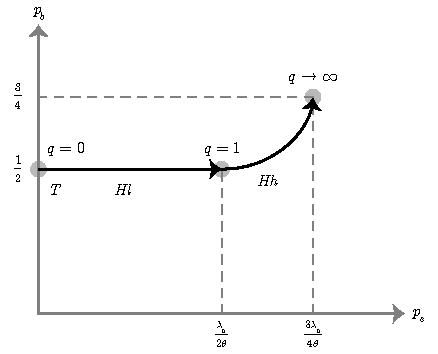
\includegraphics[width = 8.5cm]{old_figure/fig3_price_v2.pdf}
%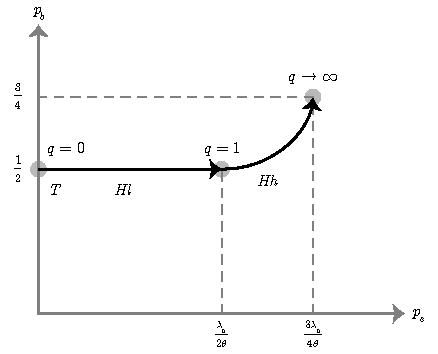
\includegraphics[scale=1.4]{old_figure/fig3_price_v2.pdf}
%\includegraphics[width=11cm]{fig3_price_v1.pdf} 
\textbf{\caption{Pricing Schemes and First-best Prices\label{fig:price}}}
\end{figure}

From this lemma, we derive how the optimal service fees of the profit-maximizing platform change according to each pricing scheme, which can be understood as the price structure with different amounts of the free bandwidth allowance. Figure 3 illustrates how the optimal fees in the first-best prices ($p_s^o, p_b^o$) change as the coefficient of the free bandwidth $q$ increases. 

First, we find that in the two-part tariff, the platform achieves the highest profit when it does not impose the storage fee (i.e., $p_s=0$) and charges the smallest bandwidth fee without any free amount of the bandwidth service. Since all bandwidth usage is subject to the bandwidth service fee in the two-part tariff, the platform is better off allowing renters to join the platform for free.

Second, when the free bandwidth amount increases (i.e., $q$ increases) for $0 \le q \le 1$, the platform's optimal service fees are achieved by increasing the storage service fee while keeping the same bandwidth service fee. This occurs when the platform offers the free-download volume below the lowest bandwidth usage level of all renters $\lambda_0$. That is, all potential renters have a higher $\lambda$ than the free bandwidth allowance and are subject to the bandwidth service fee. In this vein, the platform can exactly make up for the revenue loss by offering free downloads and increasing a lump-sum fee. As a result, all renters pay the same total service cost in this pricing scheme, as is the case of the two-part tariff.

Lastly, the platform is better off increasing $p_b$ as well as $p_s$ when the amount of free download exceeds the minimum usage $\lambda_0$, i.e., $q \in (1, \infty)$. Specifically, $q > 1$ implies that some renters enjoy the complete bandwidth service for free because their bandwidth usage levels are lower than $q \lambda_0$. Then, the platform wants to fill this cost-utility gap by increasing the storage service fee to renters. Note that the hybrid pricing becomes equivalent to the subscription-based pricing when $q \rightarrow \infty$ because all renters can use the bandwidth for free.\\

\noindent \textbf{\large Market-clearing Prices}

\noindent Now, we consider the situation where renters are rationed by the supply level due to the insufficient number of potential providers in the market compared to the storage demand from renters (i.e., \textit{the market-clearing prices}). We investigate how this supply-side restriction affects the platform's profit and system surplus for the three pricing schemes that we study in this paper.

To do so, we first investigate the required number of providers for the first-best prices. Lemma \ref{lem:threshold} summarizes this result. 

\begin{Lemma}\label{lem:threshold}
The platform's optimal service fees belong to the market-clearing prices when the number of potential providers $n_p$ is lower than the threshold $\psi$, which is calculated as:
\begin{equation*}
\begin{aligned}
    &\psi = \begin{cases}
    \frac{\xi \theta }{\alpha} n_r  &\text{ for the two-part tariff and the hybrid pricing with } q\le 1,\\
    \frac{5q^3 -3 q^2 + 3q - 2}{3q^3 + 3q^2 - 3q} \frac{\xi \theta }{\alpha} n_r   &\text{ for the hybrid pricing with } q \ge 1,\\
    \frac{5}{3}\frac{\xi \theta }{\alpha} n_r &\text{ for the subscription-based pricing,}
    \end{cases}
    \end{aligned}
\end{equation*}
and the optimal service fees of the platform decrease in $n_p$ when $n_p \le \psi$. 
\end{Lemma}

\begin{figure}[ht!]
\centering
%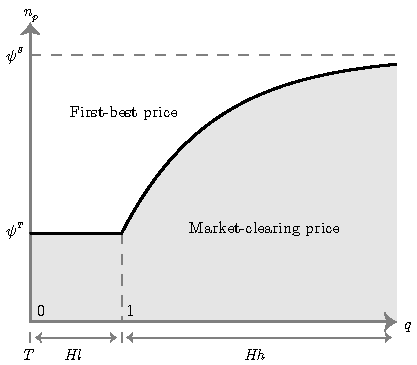
\includegraphics[scale=1.4]{old_figure/fig4_psi_v2.pdf} 
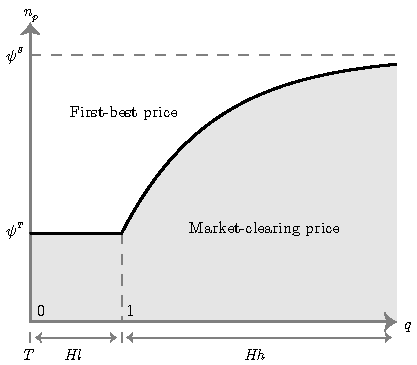
\includegraphics[width=8.5cm]{old_figure/fig4_psi_v2.pdf} 
\textbf{\caption{Free Bandwidth Allowance and First-best Price Thresholds\label{fig:first_best}}}
\end{figure}

For simplicity, we denote the thresholds of the two-part tariff and the subscription-based pricing by $\psi^T$ and $\psi^S$, respectively. Figure \ref{fig:first_best} illustrates how the first-best price threshold $n_p$ changes with respect to the coefficient of free bandwidth allowance $q$ in the hybrid pricing as shown in Lemma \ref{lem:threshold}. Specifically, when there are ample potential providers in the market compared to the threshold, the platform can achieve the highest profit using the first-best prices. Otherwise, such prices do not sufficiently incentivize providers to satisfy the storage demand from renters. As presented in Figure \ref{fig:first_best}, the threshold increases in $q$, suggesting that a high free bandwidth allowance discourages providers from participating in the platform due to a high operating cost involved with it. We also find that the threshold increases in $\xi \theta$, and it decreases in $\alpha$. Note that $\xi \theta$ is proportional to the total operating cost of providers, while $\alpha$ indicates the providers' revenue share. Therefore, these results indicate that the first-best prices become less feasible as providers' profitability decreases.

When the size of potential providers is insufficient to meet the storage demand from renters, the platform should set the market-clearing prices to incentivize providers. Specifically, for a given pricing scheme, the platform is better off by increasing both $p_s$ and $p_b$ until the number of participating providers equals the number of renters willing to adopt the platform. Alternatively, the platform may incentivize providers by lowering $q$ to fulfill the storage demand from renters (Lemma \ref{lem:threshold}). In that case, since a lower free bandwidth allowance can reduce renters' utility---particularly those with a high usage level, this approach increases service costs imposed on renters.

\begin{center}\textbf{\large Optimal Redundancy Algorithm}\end{center}

\noindent Recall that the P2P storage platform uses the redundancy rate denoted by $\theta$ and the uptime level $t$ to avoid security problems and ensure a high capacity availability. In this subsection, we consider the platform's endogenous decision on the redundancy algorithm by considering its potential consequences. The redundancy algorithm may affect the behavior of renters and providers in the following ways. First, a higher redundancy rate $\theta$ indicates that each renter contracts with a larger number of providers for the same volume of files. This incurs a higher storage cost to renters and a higher storage revenue to providers, which prohibits renters from adopting the platform. In contrast, an increase in the storage revenue encourages providers to join the platform. Second, the bandwidth volume transmitted through each provider decreases with $\theta$. As $\theta$ increases, more providers share the given bandwidth demand. Therefore, the bandwidth revenue and the operating cost for each provider decrease. Third, a higher $\theta$ leads to a lower uptime $t$ to meet the intended availability level, lowering each provider's operating cost. Here, we derive how the platform should determine the redundancy algorithm in Theorem \ref{thm:redundancy}.

\begin{Theorem}\label{thm:redundancy}
For all pricing schemes, the profit-maximizing redundancy algorithm minimizes the total providers' operating costs in the platform; that is, $\arg\max_{\theta, t} \Pi(p_s^o, p_b^o) = \arg\min_{\theta, t} \xi \theta$.
\end{Theorem}

Recall that we assume that firms only consider $(\theta, t)$ combinations that satisfy the target failure probability, as discussed in the Model Setups section, implying that $\theta > 1$ and $t > 0$. The theorem shows that the platform always decides to set the algorithm to minimize the total operating costs of providers, which is proportional to $\xi \theta$---where $\xi$ is an increasing function of uptime $t$. A lowered operating cost implies that the P2P storage network is more efficient and attractive to potential providers, which leads to a larger number of participating providers. Namely, a lower $\xi \theta$ enables the platform to serve the same number of renters with fewer potential providers and achieve the first-best prices, in line with Lemma \ref{lem:threshold}.

Furthermore, we show that the optimal ($\theta$, $t$) is identical across the pricing schemes. This result is intuitive considering that lowering operating costs helps every stakeholder, and importantly, $\xi \theta$ is not a function of service fees, storage capacity, or usage levels. Based on these findings, we can directly use Lemmas \ref{lem:pricing} and \ref{lem:threshold} to compare these pricing schemes.

\begin{center}\textbf{\large PRICING SCHEMES, PROFIT, AND SYSTEM SURPLUS}\end{center}

\noindent Since the P2P storage service uses a two-sided platform with renters and providers, it often matters whether this service improves each stakeholder's surplus. As such, two-sided platforms encounter public controversies regarding whether or not they fairly reward providers \citep{gartenberg2021google, scheiber2015growth}. Moreover, consumers and politicians are concerned about the possibility that customers are unfairly treated by large platforms \citep{kosoff2015newyorkcity}. Considering that such negative sentiments might incur substantive damages to the platform \citep{cachon2017role}, it is important to understand the potential tension between the platform's profit maximization and the other stakeholders' surplus. In this regard, we analyze the impact of pricing schemes on the overall system surplus as well as the platform's profit based on the results in the previous section.

\begin{center}\textbf{\large Under First-best Prices}\end{center}

\noindent As described in the OPTIMAL DECISIONS section, under the given service fees ($p_s, p_b$) and the total storage (paid bandwidth) volume $\upsilon_s$ ($\upsilon_{bp}$), the platform's profit $\Pi$ is:
\begin{equation*}
\Pi(p_s, p_b) = (1-\alpha) (\theta \upsilon_s p_s + \upsilon_{bp} p_b).
\end{equation*}

\noindent While providers obtain the same revenue for the storage service from renters, their operating costs differ across $\rho_j$. Thus, provider $j$ would join the platform when the costs are lower than a certain threshold; that is, $\rho_j \le \rho_m$. Also, the total providers' storage volume used by the service is $V_s = \theta \upsilon_s$. Then, the provider surplus is calculated as:
\begin{equation*}
PS = \frac{\theta \upsilon_s}{\rho_m} \int_{0}^{\rho_m} \left[ \alpha \left(p_s + \frac{\upsilon_{bp}}{\theta \upsilon_s} p_b\right) - \rho \frac{\xi \upsilon_{b}}{\theta \upsilon_s}\right] d\rho.
\end{equation*}

\noindent For renter $i$, the value from service usage is $\lambda_i u_i$ and the service cost $c_i$ depends on the pricing scheme and the service fee ($p_s, p_b$). Her surplus is then calculated as $\lambda_i u_i - c_i$. As $\lambda_i$ and $u_i$ have renter-specific value whose probability distribution functions are $f(\lambda)$ and $1$ (i.e., $u_i \sim U[0, 1]$), respectively, we calculate the total surplus of renter as:
\begin{equation*}
RS = \int_{\lambda} \int_{u(\lambda)} \{\lambda u - c(\lambda, u) \}f(\lambda) du d\lambda.  
\end{equation*}

\noindent Then, we calculate the total surplus $TS$ as the sum of the platform's profit $\Pi$, provider surplus $PS$, and renter surplus $RS$ (i.e., $TS = \Pi + PS + RS$). Using the optimal service fees in each pricing scheme under the first-best prices in Lemma \ref{lem:pricing}, we obtain the platform's profit ($\Pi$) and the total surplus ($TS$) for each pricing scheme. Theorem \ref{thm:surplus_first} below shows the order of the platform's profit and the total system surplus under the first-best prices:

\begin{Theorem}\label{thm:surplus_first} 
Under the first best prices, the orders of the platform's profit and the total surplus in the three pricing schemes are determined as follows:
\begin{table}[h] \centering
\label{tbl:thm1}
    \begin{tabular}{l  l}
        Platform's profit & $\Pi^S  \le \Pi^{Hh} \le \Pi^{Hl} = \Pi^T $\\
        %Providers' surplus & $PS^S  \le PS^{Hh} \le PS^{Hl} = PS^T $\\
        %Renters' surplus & $RS^T = RS^{Hl} \le RS^{Hh} \le RS^S$\\
        Total surplus & $TS^T = TS^{Hl} \le TS^{Hh} \le TS^S$,
    \end{tabular}
\end{table}

\noindent where the superscripts $T$, $Hl$, $Hh$, and $S$ indicate the two-part tariff, the hybrid pricing with low $q (\le 1)$, the hybrid pricing with high $q (\ge 1)$, and the subscription-based pricing, respectively.
\end{Theorem}

Notably, the two-part tariff and the hybrid pricing with low $q$ yield equivalent outcomes (i.e., $\Pi^{T} = \Pi^{Hl}$ and $TS^T = TS^{Hl}$). As discussed in Lemma \ref{lem:pricing}, the free bandwidth allowance is smaller than any usage level of renters when $q < 1$ (i.e., $q\lambda_0 < \lambda_0$). Therefore, the platform under the hybrid pricing with low $q$ can increase $p_s$ up to the level where the platform can recover the revenue reduction from the bandwidth service without losing renters. In this way, the platform can achieve the same revenue under the two-part tariff even when they offer a limited free bandwidth allowance.

In contrast, an increase in $q$ above 1 lowers the profit of the platform (i.e., $\Pi^{Hh} \le \Pi^{Hl}$) and leads to a higher total surplus (i.e., $TS^{Hh} \ge TS^{Hl}$). The free bandwidth allowance above $\lambda_0$ enables some renters to use the entire bandwidth without the bandwidth service cost. To charge these renters, the platform would raise the storage service fee. Still, this does not fully recover the revenue loss from free-download volume from renters. In practice, firms are likely to consider offering `meaningful' instead of `negligible' amounts of free usage to attract customers. In this sense, our results imply that P2P storage platforms have little incentive to leverage the free allowance to improve their short-term profits. Note that the subscription-based pricing, which offers the unlimited free bandwidth allowance, can be understood as an extreme case of hybrid pricing. As $q$ increases further and goes to infinity, the platform obtains the lowest profit, and the system surplus reaches its highest value.

Remarkably, all pricing schemes attract the same number of renters to the platform under the first-best prices. Therefore, the differences in the total surplus are mainly driven by the difference in the usage level of renters instead of the total size of renters. Specifically, as $q$ increases, renters with a higher usage level $\lambda$---who gain a relatively high utility compared to those with a lower $\lambda$---are more likely to adopt the platform. In this way, the renters' benefit from an increase in $q$ outweighs the loss of profits, which increases the system surplus.

\begin{center}\textbf{\large Under Market-clearing Prices}\end{center}

\noindent The consequences of pricing schemes under the market-clearing prices are less straightforward than the first-best prices because service fees can indirectly interact with renter decisions through altering the supply level. We account for this interaction and obtain the following results.

\begin{Theorem}\label{thm:surplus_market}
When the first-best price is not feasible for some pricing schemes, there exist $\underline{\psi}$ as the size of potential providers that satisfy $0 \le \underline{\psi} \le \psi^T < \psi^S$. Then, the platform's profit and total surplus in the three pricing schemes have the following orders.
\begin{enumerate}[label=(\roman*)]
    \item When $n_p$ is moderate such that $\psi^T \le n_p \le \psi^S$, hybrid pricing with $q \ge 1$ can dominate the subscription-based pricing, i.e., $\Pi^{Hh} \ge \Pi^S$ and $TS^{Hh} \ge TS^S$.
    \item When $n_p$ is small such that $\underline{\psi} \le n_p \le \psi^T $, the two-part tariff and hybrid pricing with $q \le 1$ yield higher total surplus than the subscription-based pricing; that is, $TS^T = TS^{Hl} \ge TS^S$. Also, these pricing schemes always ensure higher profits than the subscription-based pricing; that is, $\Pi^T = \Pi^{Hl} \ge \Pi^S$.
\end{enumerate} 
\end{Theorem}

% \begin{Theorem}\label{thm:surplus_market}
% When the first-best price is not feasible for some pricing schemes, there exist $\underline{\psi}$ as the size of potential providers that satisfy $0 \le \underline{\psi} \le \psi^T < \psi^S$. Then, the platform's profit and total surplus in the three pricing schemes have the following orders.
% \begin{enumerate}[label=(\roman*)]
%     \item When $n_p$ is moderate such that $\psi^T \le n_p \le \psi^S$, a hybrid pricing with $q \ge 1$ can dominate the subscription-based pricing, i.e., $\Pi^H \ge \Pi^S$ and $TS^H \ge TS^S$.
%     \item When $n_p$ is small such that $\underline{\psi} \le n_p \le \psi^T $, the two-part tariff dominates the subscription-based pricing; that is, $\Pi^T \ge \Pi^S$ and $TS^T \ge TS^S$.
% \end{enumerate} 
% \end{Theorem}

Theorem \ref{thm:surplus_market} suggests that the effectiveness of pricing schemes is highly contingent upon the number of potential providers $n_p$ in the market. When $n_p$ is large such that $n_p \ge \psi^S $, the platform can set the first-best prices. Hence, all results in Theorem \ref{thm:surplus_first} hold, and the subscription-based pricing---which creates the renter surplus most---always yields the highest total surplus. However, as $n_p$ decreases, the first-best prices become insufficient to incentivize providers. Hence, the platform should give a higher reward to each provider to maintain the same level of capacity. This result indicates that the size of potential providers needs to be carefully considered in the platform's pricing decisions. 

We further investigate how the optimal service fees in the pricing schemes interplay with $n_p$ and find the following results. First, as $n_p$ is moderate such that $\psi^T \le n_p \le \psi^S$, there exists some hybrid pricing with $q \ge 1$ that outweighs the subscription-based pricing in terms of the total surplus as well as the platform's profit. As suggested by Lemma \ref{lem:threshold}, the first-best prices are not applicable for the subscription-based pricing when $n_p$ is moderate. Hence, the profit-seeking platform needs to adopt the market-clearing prices to incentivize providers and avoid rationing renters who are willing to pay for the service. Thus, the subscription-based pricing experiences a significant decline in the platform's profit, the provider surplus, and the renter surplus. Alternatively, the platform may achieve the first-best prices by reducing the free bandwidth allowance. By balancing the incentive for providers and the renters' utility from the free bandwidth allowance, the platform can achieve a higher total surplus when the number of potential providers is comparable to the number of potential renters.

Second, we show that the two-part tariff, which is equivalent to hybrid pricing with $q \le 1$, can yield the higher surplus than the subscription-based pricing when $n_p$ is small such that $\underline{\psi} \le n_p \le \psi^T $. In this case, the platform should attract a large proportion of potential providers to meet the same storage demand from renters. Then, the free bandwidth allowance affects the platform's ability to fulfill the storage demand more adversely. The platform needs to set strikingly high subscription fees to compensate for this adverse effect, and consequently, the renter surplus---the main advantage of the subscription-based pricing---substantially decreases. In contrast, the two-part tariff can maintain the required capacity for market-clearing with relatively cheap service fees because it rewards providers for all bandwidth provision. As a consequence, the two-part tariff can achieve a higher system surplus than the subscription-based pricing, implying that rewarding providers could be more beneficial to the entire system than focusing on the renter surplus.

Concerning the profit comparison, we provide closed-form evidence that two-part tariff, hybrid with $q \le 1$, and subscription-based pricing schemes have the equivalent order between Theorem \ref{thm:surplus_first} and Theorem \ref{thm:surplus_market}. We further investigate the relative profit of hybrid pricing with $q \ge 1$ compared with those of the other pricing schemes. From numerical analyses throughout wide parameter ranges, we observe that the relative profits decrease with free bandwidth $q$, which is consistent with the findings from Theorem \ref{thm:surplus_first}.\footnote{The results of numerical analysis are available upon request. For the peer-review process, we can provide the results as a separate material. Please reach out to the authors indirectly through the editors.}


\begin{center}\textbf{\large MODEL EXTENSION AND DISCUSSION}\end{center}

\begin{center}\textbf{\large Assumptions on the Platform}\end{center}
% Endogenous Decision on Commission Rates

\noindent Thus far, we have assumed an exogenously given commission rate when investigating the platform's optimal service fees. Although it is difficult for two-sided platforms to alter commissions because they often encounter public controversies regarding whether or not they fairly reward providers \citep{gartenberg2021google, scheiber2015growth}, it is still informative to understand how the implications of pricing schemes change when the platform is free to adjust its commission rate. Therefore, in this subsection, we consider an endogenously determined commission rate of the platform. Now, the platform can choose a commission rate to better maximize its profit. Also, it is possible that such a benefit may be amplified under a non-flexible pricing scheme (e.g., the subscription-based pricing). To verify the possibility that the endogenous selection of commission rates affects our findings, we re-analyze our model by considering $\alpha$ as a decision variable as well as $p_s$ and $p_b$. Theorem \ref{thm:alpha} summarizes the results according to the exogenous size of potential providers $n_p$. 

\begin{Theorem}\label{thm:alpha}
If the profit-seeking platform endogenously determines the commission rate, there exists $\bar{\psi}_{\alpha}$ as the size of potential providers that satisfies $0 \le \psi_{\alpha}^T \le \bar{\psi}_{\alpha} \le \psi_{\alpha}^S$, where $\psi_{\alpha}^T \equiv \frac{1}{2}\xi \theta n_r$ and $\psi_{\alpha}^S \equiv 3 \xi \theta n_r$. Then, the platform's profit and the total surplus in the three pricing schemes have the following orders.
\begin{enumerate}[label=(\roman*)]
    \item When $n_p$ is large such that $n_p \ge \bar{\psi}_{\alpha}$, the two-part tariff generates the highest platform's profit, while the subscription-based pricing yields the highest total surplus (Theorem \ref{thm:surplus_first}).
    \item When $n_p$ is moderate such that  
    $\psi_{\alpha}^T \le n_p \le \bar{\psi}_{\alpha}$, hybrid pricing with some $q \ge 1$ dominates the subscription-based pricing. That is, $\Pi^{Hh} \ge \Pi^S$ and $TS^{Hh} \ge TS^S$ (Theorem \ref{thm:surplus_market} (\textit{i})),
    \item When $n_p$ is small such that $0 \le n_p \le \psi_{\alpha}^T$, the two-part tariff and hybrid pricing with $q \le 1$ yield higher total surplus than the subscription-based pricing; that is, $TS^T = TS^{Hl} \ge TS^S$. Also, these pricing schemes always ensure higher profits than the subscription-based pricing; that is, $\Pi^T = \Pi^{Hl} \ge \Pi^S$ (Theorem \ref{thm:surplus_market} (\textit{ii})).
\end{enumerate}
\end{Theorem}

% \begin{Theorem}\label{thm:alpha}
% If the profit-seeking platform endogenously determines the commission rate, there exists $\bar{\psi}_{\alpha}$ as the size of potential providers that satisfies $0 \le \psi_{\alpha}^T \le \bar{\psi}_{\alpha} \le \psi_{\alpha}^S$, where $\psi_{\alpha}^T \equiv \frac{1}{2}\xi \theta n_r$ and $\psi_{\alpha}^S \equiv 3 \xi \theta n_r$. Then, the platform's profit and the total surplus in the three pricing schemes have the following orders.
% \begin{enumerate}[label=(\roman*)]
%     \item When $n_p$ is large such that $n_p \ge \bar{\psi}_{\alpha}$, the two-part tariff generates the highest platform's profit, while the subscription-based pricing yields the highest total surplus (Theorem \ref{thm:surplus_first}).
%     \item When $n_p$ is moderate such that  
%     $\psi_{\alpha}^T \le n_p \le \bar{\psi}_{\alpha}$, a hybrid pricing with some $q \ge 1$ dominates the subscription-based pricing. That is, $\Pi^H \ge \Pi^S$ and $TS^H \ge TS^S$ (Theorem \ref{thm:surplus_market} (\textit{i})),
%     \item When $n_p$ is small such that $0 \le n_p \le \psi_{\alpha}^T$, the two-part tariff dominates the subscription-based pricing. That is, $\Pi^T \ge \Pi^S$ and $TS^T \ge TS^S$ (Theorem \ref{thm:surplus_market} (\textit{ii})).
% \end{enumerate}
% \end{Theorem}

The theorem shows that our main insights obtained in Theorems \ref{thm:surplus_first} and \ref{thm:surplus_market} continue to hold, although the thresholds for the first-best prices change. This suggests that it is still crucial for the platform to incentivize providers, even when it is free to alter its commission rate to increase its own profit.

Although the results from endogenous commission rates are consistent with our main findings, we should interpret them with caution for the following reasons. First, two-sided platforms need to carefully consider public sentiment as well as their profits because they often encounter public controversies regarding whether they fairly reward providers \citep{gartenberg2021google, scheiber2015growth}. Second, potential competition and regulations might inhibit platforms from choosing the high commission rates they wish to providers. Even when competitors are not strong or even absent, unsatisfactory rewards for storage supply might encourage new entrants to grow their shares in the market. Lastly, the suggested commission rates might be unrealistic. Sia's commission rate is about 3.9\%, and mobile app stores---i.e., Google Play and Apple's App Store---charge 30\% to app providers. Considering the fierce resistance to 30\% commission rates in app markets \citep{gartenberg2021google}, 67\% or higher commission rates might not be a viable option. For these reasons, the assumption of exogenous commission rates can be reasonably acceptable in our context.

\begin{center}\textbf{\large Assumptions on Providers}\end{center}

% R1's Point 1 (Redundancy's feasibility)
%We have made several assumptions about providers and renters, which might have driven our findings. 
\noindent In this subsection, we discuss the plausibility and potential consequences of assumptions on providers, and if applicable, we conduct numerical analyses to quantitatively examine these issues. Specifically, our model excludes the case where operating costs are negligible for potential providers; that is, we assume that $\xi > \frac{3}{4} \alpha$. Although online forums for P2P storage platforms have been significantly concerned the profitability and operating costs, it is still insightful to understand the consequences of pricing schemes when operating costs become negligible. We conduct a numerical study examining how small operating costs (i.e., $\xi \le \frac{3}{4} \alpha$) can affect our results and report the results in Appendix \ref{app:numerical}. Below, we summarize key insights from this analysis.

When $\xi$ is substantially small (i.e., low operating costs), all potential providers are willing to share their storage and participate in the platform. Since providers do not respond to bandwidth fees sensitively under small $\xi$, raising prices does not help renters find more capacity while it increases their financial burden. Therefore, the two-part tariff and the hybrid pricing, which compensate for providers' bandwidth services, are less effective in boosting system surplus than the subscription-based pricing. Consequently, the surplus implication of pricing schemes is similar to the first-best prices under substantially small $\xi$.

% R2's Point A2b (Proportional operating costs/storage volume heterogeneity)
Second, it is possible that providers have a different cost distribution, which can determine how much they are willing to share storage and bandwidth volumes. Specifically, individuals may have different storage costs, leading to heterogeneous storage capacities in P2P networks. Under such heterogeneous capacities, an alternative form of the provider's operating costs may raise a concern about the validity of our findings. For now, our functional form relies on the assumptions that operating costs are proportional to $\hat{\omega_b}$ (i.e., the expected bandwidth volume for each provider), and that $\hat{\omega_b}$ is proportional to each provider's shared storage capacity. We argue that these assumptions are plausible for the following reasons: 1) many of the major costs, such as Internet bandwidth and electricity costs, are proportional to bandwidth usage, and 2) the platform tends to assign more files and bandwidth services to high-capacity providers than low-capacity ones.

So, how would alternative cost forms affect the results? On the one hand, we may consider a convex function, such as quadratic and exponential forms, where operating costs are particularly burdensome for high-capacity providers. In this case, as high-capacity providers bear much higher operating costs and join the platform less, compensating for offering bandwidth services will have a higher impact on the storage capacity. Consequently, the relative benefits of two-part tariff and hybrid pricing (vs. subscription-based pricing) will be greater in this situation. On the other hand, we may also consider a concave function like a square root function. Since high-capacity providers bear relatively less operating burden than they do in the current setup, the platform will attract more providers under the subscription-based pricing. Hence, the profit/surplus gap between the subscription and other pricing schemes will decrease as a result. However, although the magnitudes decline, we expect the differences to remain qualitatively unchanged.

% R2's Point A3 (Informed decision)
Third, and importantly, one might wonder if providers can meaningfully predict the demand for storage and bandwidth services in advance. We argue that providers can make informed choices based on multiple sources that offer information before joining the platform. For example, individual providers have actively analyzed and shared their profitability in online forums, such as Reddit. Also, the P2P storage platforms notice their minimum requirement and recommended capacity of computing resources before individuals decide to join their networks. Such information can partially inform them about their expected operational costs. They also publicize their storage sharing status, such as used storage, number of transactions, network revenues, and hash rates (e.g., SiaStats). Moreover, even when unsuccessful on the platform, they can quickly leave the network, similar to other digital markets. In sum, due to the platform-offered information, online forums, and easiness of market entry/exit, we expect that participants in the platform will rapidly reach market equilibrium.

\begin{center}\textbf{\large Assumptions on Renters}\end{center}

\noindent In this subsection, we investigate the potential consequences of  assumptions on renters. Specifically, we conduct numerical analyses on our assumptions on renter heterogeneity and present the results in Appendix \ref{app:numerical}. We find the following main insights. First, our numerical experiments suggest that our findings remain consistent when we relax the assumption of bandwidth usage distribution of renters.\footnote{For this result, we assume that bandwidth usage follows the Pareto distribution with $b=2$ to account for the heavy-tail distribution and analytical tractability. To assess whether this assumption is entirely responsible for our findings, we conduct a numerical analysis of different shapes of distributional tails. For ease of comparison, we have varied the Pareto’s shape parameters and tested whether our findings continue to hold.} The results indicate that the implications of pricing schemes do not change under different parametric conditions. Second, our model postulates that the distributions of the utility per bandwidth volume and the download frequency are independent. Although this leads to a positive association between these variables as a result of self-selection, it is also possible that they are positively associated with each other before the renter's decision. We observe that our main findings remain qualitatively consistent.

Third, we further consider an additional dimension of heterogeneity: storage demand. One may be concerned that our assumption of homogeneous storage demand may have driven our findings. In particular, pricing schemes might have unexpected influences if their storage and bandwidth needs are correlated. To assess this possibility, we conduct numerical analyses utilizing various distributions of storage and bandwidth volumes. We observe that the main insights from the basic setup remain qualitatively unchanged in our results.\footnote{However, when we allow some renters to have more storage demand than the unit volume, a larger share of renters may need more bandwidth capacity than the bandwidth allowance. Consequently, the influence of hybrid pricing becomes similar to that of a two-part tariff, altering the boundaries in Theorem \ref{thm:surplus_market}.}

Importantly, we observe from our several numerical analyses that firms can achieve a higher surplus from $Hh$-type hybrid pricing only if either operating costs are extremely low or sufficiently large potential providers (vs. potential renters) exist. Therefore, a two-part tariff is likely the most desirable option, even for the total surplus with a small provider base.

\newpage

\begin{center}\textbf{\large CONCLUSIONS}\end{center}

% Research summary
\noindent In this study, we developed a game-theoretic model to examine how the P2P storage platform's pricing schemes impact the platform's profit and the total system surplus. We considered three pricing schemes, one of which is widely employed by P2P storage platforms (the two-part tariff) while the others are widely adopted by conventional public cloud services (the subscription-based pricing and the hybrid pricing). Also, we incorporated endogenous decisions on redundancy algorithms into deciding profit-maximizing service fees under a given pricing scheme.

We showed that when the first-best prices---which maximizes the platform's profit when the number of potential providers is sufficient---are applicable, the two-part tariff outperforms the other pricing schemes in terms of profit maximization, while the subscription-based pricing surpasses the others regarding the total surplus. Remarkably, we revealed that the relative influences of pricing schemes significantly change when the scarcity of potential providers is considered. When potential providers are not sufficient to meet the storage demand, the platform cannot set the first-best prices. Instead, it should employ the market-clearing prices wherein the supply and demand become equivalent. In this case, the two-part tariff and the hybrid pricing may dominate the subscription-based pricing regarding both the profit and the total surplus. To further validate our findings, we examined how endogenous commission rates and relaxing other assumptions affect the results. We found that our key findings remain qualitatively unchanged.

Our findings are attributable to the decentralized nature of two-sided platforms. Considering that a two-part tariff can decide both a rump-sum fee and a per-use fee, unlike pay-per-use only in some papers---e.g., \citet{randhawa2008usage}, \citet{cachon2011pricing}, it is intuitive that a firm can convert renter surplus into its profit under two-part tariff than subscription-based pricing. Also, we obtain a higher total surplus from subscription-based pricing under an abundant storage supply, where pricing decisions have a limited impact on the supply level, as expected by the extant literature. In this sense, our finding of when and why the platform's seemingly `greedy' choice may benefit both sides of platform participants is not contradictory to the literature but offers unique insights into P2P markets.

% Managerial implications for P2P storage platforms
Our findings provide numerous implications for P2P storage platforms that rely on independent suppliers and concern the surplus of stakeholders. We compared the currently adopted pricing scheme with other pricing schemes rarely used by the P2P storage platforms and revealed that the scarcity of potential providers plays a central role in determining the effects of pricing schemes. Specifically, we showed that if there is a sufficiently large base of potential suppliers, the platform can enhance the total surplus of the system by adopting the subscription-based pricing instead of the two-part tariff. On the other hand, if the size of potential providers is not sufficient, the subscription-based pricing might lead to a lower surplus than the two-part tariff and the hybrid pricing, which ensure the higher profit for the platform. In addition, our results suggest that the effectiveness of a pricing scheme substantially interplays with the redundancy algorithm. Specifically, the two-part tariff and the hybrid pricing become increasingly effective as the redundancy algorithm requires a higher uptime and redundancy rate, raising providers' operating costs.

In this vein, our findings provide actionable insights that these platforms can directly apply. Given the immature stage of the P2P storage market, the platforms might want to expand the user base by increasing the total system surplus rather than seeking its short-term profit only. In doing so, they may consider adopting alternative pricing schemes that can yield a higher surplus than the two-part tariff. However, it could be demanding to attract potential providers to the platform, perhaps due to technical difficulties of sharing computing resources. If so, the P2P storage platform needs to further compensate providers' bandwidth provision rather than their storage capacity by lowering the free bandwidth allowance. It is worth noting that Storj introduced a new pricing scheme wherein renters receive a finite amount of free usage volume. Our results suggest that this change can hardly be supported from a profit-seeking perspective in the short term. Also, based on several numerical analyses, we observe that the firm is likely to achieve a higher total surplus only if both the free volume and the potential size of providers are substantial. Therefore, the current choice might not necessarily help its P2P network flourish.

It is also possible that the platform cannot alter its pricing scheme and service fees. In that case, the platform may indirectly incentivize providers by requiring a lower uptime or a lower redundancy rate. For instance, a $k$-of-$m$ erasure coding scheme with the same redundancy rate (i.e., the same $\frac{m}{k}$) can achieve the same availability while reducing its required uptime by increasing $k$ and $m$ at the same time.

% Managerial implications for other types of platforms
Our research also provides managerial insights that other sharing platforms can also consider. We found that pricing schemes that further compensate providers can improve the total surplus when the size of potential suppliers is relatively more scarce than consumers. Although other platforms often employ different pricing schemes, the underlying intuition could be similarly applied to these platforms. We showed that a rise in service prices could mitigate this situation where only a few providers endure high operating costs. In this regard, sharing platforms may consider heterogeneous pricing strategies across regions. For example, peer-to-peer delivery platforms serve various regions with different sizes of sellers, deliverers, and consumers. In regions where relatively scarce deliverers are bearing the delivery costs, the platforms may achieve not only higher profits but also a higher surplus of all stakeholders by further charging sellers/consumers. In contrast, the system surplus will be increased by lowering service prices when sufficient deliverers are in the regions.

%(P5) Limitation and future research
We conclude by specifying some caveats and potential avenues for future research. First, we have analyzed only a monopoly market. The P2P storage market is highly immature and still rapidly growing, and several new entrants are threatening incumbent players. We expect that future research can significantly benefit from investigating the influence of competitors in this nascent market. Second, our model relies on a homogeneous storage volume in order to focus on the interactions between renters and providers. Although the numerical analysis suggests that our findings are insensitive to renter's heterogeneous storage, future studies can make substantial progress by incorporating the heterogeneity of storage volume from the supply and demand sides into their main models. Moreover, our model does not consider the possibility that renters may change their usage levels depending on pricing schemes, which can provide a valuable direction for future research. Third, it is also worth mentioning that we do not provide the closed-form results of welfare comparison completely. Although our numerical results showed a general tendency that a two-part tariff yields a higher surplus than hybrid pricing with a large free bandwidth allowance, future studies may provide better insights by comparing these pricing schemes more comprehensively. Lastly, our results are restricted to three pricing schemes, but many other pricing schemes can be considered. For instance, some public cloud services lower the unit price as the usage level increases in practice. Moreover, cloud platforms may consider offering multiple pricing schemes to differentiate various customer segments more effectively. Analyzing how unexplored pricing schemes affect the platform’s profit and system surplus can provide valuable insights.

\setlength{\baselineskip}{14pt}
\setlength{\bibsep}{0pt plus 0.3ex}
    %\bibliographystyle{misqref}
    \bibliographystyle{informs2014}
    %\bibliographystyle{apacite}
    %\bibliographystyle{pomsref}
    \bibliography{bib}

\setlength{\baselineskip}{22pt}
\appendix

\section{Numerical Analyses}\label{app:numerical}
%
%
\subsection{Assumptions on Providers}

% Provider assumption
% i) $\xi$가 낮은 경우\\
% i-1) $\frac{3}{4}\alpha \le \xi$가 되는 경우 어떻게 되는지\\
% i-2) 극단적으로 $\xi$가 작아지는 경우에는 어떻게 되는지\\
% i-3) 그 경우들에 대한 numerical study

% Renter assumption
% ii) Pareto distribution의 general b (tail이 작아지는 경우)
% iii) Correlation\\
% iv) Heterogeneous volume\\

% \noindent \textbf{When are previous solutions not optimal?} \\
% We have identified the conditions where our previous solutions are optimal or not as follows:\\
% \noindent \textit{Case }1) when $\frac{3}{4}\alpha \le \xi$, our all previous solutions for all pricing schemes are optimal,\\
% \textit{Case }2) when $\frac{3}{10}\alpha \le \xi < \frac{3}{4}\alpha$, some of our previous solutions for some pricing schemes cannot be optimal,\\
% \textit{Case }3) when $\xi < \frac{3}{10}\alpha$, all of our previous solutions are not optimal.
% \begin{proof} 
% To find when our previous solutions are not optimal, we are enough to find that the threshold $\bar \xi^i$ which satisfies $\pi|_{\rho_j=1} = 0$ where $i \in \{T, H, S\}$. Then, that $\bar \xi^i$ satisfies the following equation:
% \begin{equation*}
% \begin{aligned}
%     \bar \xi^i= \frac{\alpha}{\hat{\omega}_b}(\hat{\omega}_s p_s + \hat{\omega}_{bp} p_b) = \frac{\alpha}{\upsilon_b}(\theta \upsilon_s p_s + \upsilon_{bp} p_b)  = \frac{\alpha}{(1-\alpha)\upsilon_b} \Pi^i
% \end{aligned}
% \end{equation*}
% Since $\Pi^T \ge \Pi^H \ge \Pi^S$ and $\upsilon_b^T \le \upsilon_b^H \le \upsilon_b^S$ holds, the $\bar \xi^T \ge \bar \xi^H \ge  \bar \xi^S$ holds for given $n_p$ where each $\bar \xi^i$ represents the threshold.\\
% i) In order to find the maximum $\bar \xi$ that makes some previous solutions not optimal, we are enough to find the maximum value of $\xi$ that makes the previous solution not optimal when the platform selects a two-part tariff pricing scheme.\\
% According to our solutions in the main analysis, the platform sets the first-best price when $\frac{\xi \theta}{\alpha} n_r \le n_p$, and the platform sets the market-clearing price when $0 \le n_p \le \frac{\xi \theta}{\alpha} n_r$. Now, let us divide the following two cases to derive the condition when our previous solutions cannot be optimal.\\
% i-i) $\frac{\xi \theta }{\alpha} n_r \le n_p$\\
% In this case, the platform sets the first-best price and the optimal prices become
% \begin{equation*}
%     \left(p_s^T, p_b^T\right) = \left(0, \frac{1}{2}\right)
% \end{equation*}
% Then, by putting $\left(p_s^T, p_b^T\right)$ into the $\rho_m$, we get $\rho_m|_{p_s = p_s^T, p_b = p_b^T} = \frac{\alpha}{2\xi}$. Which implies that, when $\frac{1}{2}\alpha \le \xi$ holds, the first-best price becomes the optimal solution.\\
% i-ii) $0 \le n_p \le \frac{\xi \theta}{\alpha}n_r$\\
% In this case, the platform sets the market-clearing price, but the optimal prices distinguish in two cases according to the number of providers as follows.\\
% i-ii-i) $\frac{1}{6}\frac{\xi \theta}{\alpha}n_r \le n_p \le \frac{\xi \theta}{\alpha}n_r$\\
% In this case, We obtain the following optimal prices for this case.
% \begin{equation*}\small
% \begin{aligned}
%     &\left(p_s^T, p_b^T\right) = \left(\frac{3(12\eta^2 + 28 \kappa \xi - \kappa^2) - 3(2\eta + \kappa)\sqrt{180\eta^2 - 12 \kappa \eta + \kappa^2}}{8 (12\eta^2 + 12 \kappa \eta - \kappa^2)} \frac{\lambda_0}{\theta}, \frac{12\eta^2 + 24 \kappa \eta - 3\kappa^2 + \sqrt{180\eta^2 - 12 \kappa \eta + \kappa^2}}{4(12\eta^2 + 12\kappa \eta - \kappa^2)}\right)\\
%     &\text{where } \kappa = \frac{\xi}{\alpha} \text{ and } \eta = \frac{n_p}{\theta n_r}
% \end{aligned}
% \end{equation*}
% By putting above optimal prices into the threshold $\rho_m$, we get the following equations.
% \begin{equation*}
%     \rho_m^T \equiv \rho_m|_{p_s= p_s^T, p_b = p_b^T} = \frac{3(24 \eta - 4 \kappa) +6\sqrt{180 \eta^2 - 12 \kappa \eta + \kappa^2}}{12(12\eta^2 + 12 \kappa \eta - \kappa^2)}
% \end{equation*}
% Above $\rho_m^T$ has following characteristics:\\
% i) $\rho_m^T$ is maximized at $\eta = \frac{\kappa}{6}$,\\
% ii) $\rho_m^T$ decreases in $\eta$ (i.e., decreases in $n_p$) for $\frac{\kappa}{6} \le \eta \le \kappa$,\\
% iii) $\rho_m^T|_{\eta = \kappa} = \frac{1}{2 \kappa}$.\\
% These three characteristics imply that, $\rho_m^T \le 1$ holds when $\xi \ge \frac{3}{4}\alpha$.

% i-ii-ii) $0 \le n_p \le \frac{1}{6}\frac{\xi \theta}{\alpha} n_r$\\
% We obtain the following optimal prices for this case.
% \begin{equation*}
%     \left(p_s^T, p_b^T\right) = \left(\frac{\sqrt{6 \kappa }}{16\sqrt{\eta}}\frac{\lambda_0}{\theta }, \frac{5}{8} \right)
% \end{equation*}
% By putting above optimal prices into the threshold $\rho_m$, we get the following equations.
% \begin{equation*}
% \rho_m^T \equiv \rho_m|_{p_s= p_s^T, p_b =p_b^T} = \frac{3\alpha}{4 \xi}
% \end{equation*}
% Thus, when $\xi \ge \frac{3}{4}\alpha$, $\rho_m^T \le 1$ holds.

% Combining above results, we get the desired result.\\

% ii) On the other hand, we can find a threshold $\bar \xi^S$ that makes all previous solutions cannot be optimal when $\xi \le \bar \xi^S$ holds.\\
% ii-i)  Optimal $\rho_m = \frac{3\alpha}{10\xi} \rightarrow \rho_m > 1 \Leftrightarrow \xi < \frac{3 }{10} \alpha$\\
% ii-ii) Market clearing\\
% Optimal $\rho_m = \frac{\theta n_r ( 3\alpha n_p - \xi \theta n_r)}{3 n_p (\alpha n_p + \xi \theta n_r)} \rightarrow \rho_m > 1 \Leftrightarrow \frac{n_r \theta(3\alpha - 3\xi) - \sqrt{9\xi^2 - 30 \alpha \xi + 9 \alpha^2}}{6\alpha} \le n_p \le \frac{n_r \theta (3\alpha - 3 \xi) +\sqrt{9\xi^2 - 30 \alpha \xi + 9\alpha^2}}{6\alpha}$.\\
% It can be a feasible region when $\xi \le \frac{1}{3}\alpha$.\\

% Thus, when $\xi \le \frac{3}{10}\alpha$, all of our previous solutions cannot be optimal solution.

% 1) Subscription: $\rho_m = \frac{3\alpha }{10 \xi} \rightarrow \rho_m > 1 \Leftrightarrow \xi < \frac{3 \alpha}{10}$\\
% Case with $n_p$\\
% i) Subscription:\\
% i-i) First-best price\\
% Optimal $\rho_m = \frac{3\alpha}{10\xi} \rightarrow \rho_m > 1 \Leftrightarrow \xi < \frac{3 }{10} \alpha$\\
% i-ii) Market clearing\\
% Optimal $\rho_m = \frac{\theta n_r ( 3\alpha n_p - \xi \theta n_r)}{3 n_p (\alpha n_p + \xi \theta n_r)} \rightarrow \rho_m > 1 \Leftrightarrow \frac{n_r \theta(3\alpha - 3\xi) - \sqrt{9\xi^2 - 30 \alpha \xi + 9 \alpha^2}}{6\alpha} \le n_p \le \frac{n_r \theta (3\alpha - 3 \xi) +\sqrt{9\xi^2 - 30 \alpha \xi + 9\alpha^2}}{6\alpha}$.\\
% It can be a feasible region when $\xi \le \frac{1}{3}\alpha$.\\

% Solution:\\
% i) Subscription:\\
% i-i) $0 \le p_s \le \frac{\lambda_0}{\theta}$\\
% $p_s^* = \frac{3 \lambda_0 (n_r - n_p )}{2\theta n_r} \rightarrow p_s^* \le \frac{\lambda_0}{\theta} \Leftrightarrow n_p \ge \frac{n_r}{3}$\\
% i-ii) $\frac{\lambda_0}{\theta}\le p_s $\\
% $p_s^* = \frac{\sqrt{n_r}}{\sqrt{3n_r}} \frac{\lambda_0}{\theta} \rightarrow p_s^* \ge \frac{\lambda_0}{\theta} \Leftrightarrow n_p \le \frac{n_r}{3}$\\

% ii) In order to find the maximum $\xi$ that makes all previous solutions not optimal, we are enough to find the $\xi$ that makes the all previous solution not optimal when the platform selects a subscription pricing scheme.\\
% According to our solutions in the main analysis, the platform sets the first-best price when $\frac{5\xi\theta}{3\alpha}n_r \le n_p$, and the platform sets the market-clearing price when $0 \le n_p \le \frac{5 \xi \theta}{3\alpha}n_r$. Now, let us divide the following two cases to derive the condition when our previous solutions cannot be optimal.
% ii-i) 

% R1's Point 1 (Redundancy's feasibility)
Our model only considers the case where operating costs are not negligible for potential providers; that is, we assume that $\xi > \frac{3}{4} \alpha$. In this analysis, we examine how the implications of the pricing schemes change when operating costs are negligible or $\xi \le \frac{3}{4} \alpha$. \textbf{Figure \ref{fig:app_lowxi}} depicts the numerical analysis results. The graph presents the relative system surplus of the two-part tariff (the red line) and hybrid pricing (the blue line) under $\xi = 0.2$, $b=2$, $q=2$, $\theta=3$, $\alpha=0.95$, and $\lambda_0=1$.

We have found that the subscription-based pricing outperforms the two-part tariff and the hybrid pricing in any small $\xi$ in this case (i.e., operating costs decrease). Since providers do not respond to bandwidth fees sensitively under small $\xi$, raising prices does not help renters find more capacity while it increases their financial burden. Therefore, the two-part tariff, which compensates for providers' bandwidth services, becomes less effective in boosting system surplus than the subscription-based pricing. Consequently, the surplus implication of pricing schemes is similar to the first-best prices under substantially small $\xi$. The small $\xi$ affects the surplus implication of the hybrid pricing similarly.

\setcounter{figure}{0}
\begin{figure}[ht!]
\centering
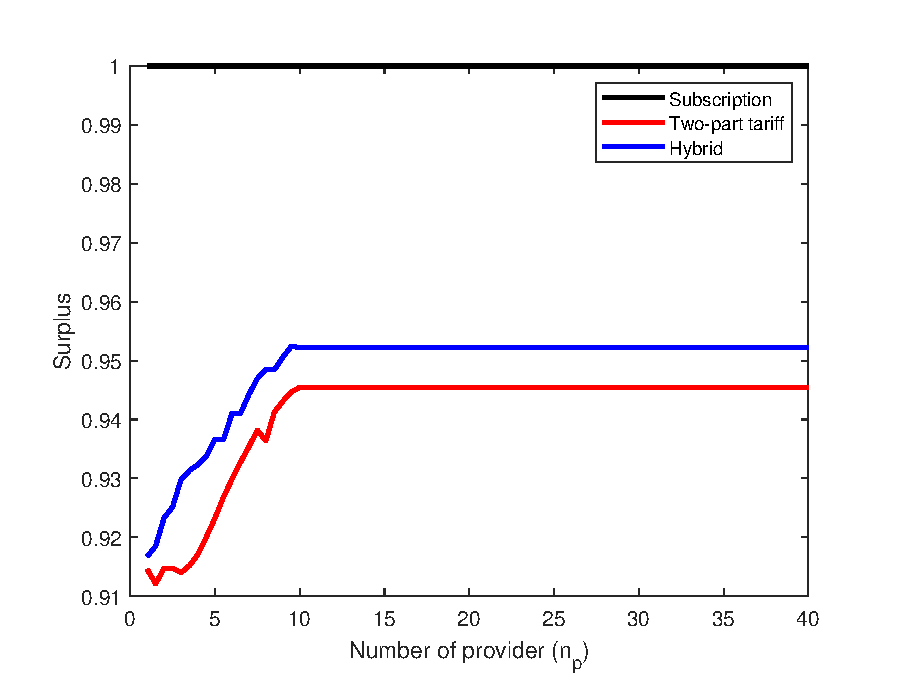
\includegraphics[width=8cm]{figure_3rd_final/f_low.eps} 
\textbf{\caption{Surplus Comparison for Extremely Low Operating Costs}}
\label{fig:app_lowxi}
\end{figure}

\subsection{Assumptions on Renters}
 
We conduct a numerical analysis for different shapes of the download frequency distribution. We vary the Pareto's shape parameter $b$ by three levels ($b=3, 4, \text{or } 5$) and present the results in \textbf{Figure \ref{fig:app_pareto}}. Here, the red (blue) line indicates the relative total surplus of the two-part tariff (the hybrid pricing) compared with the subscription-based pricing, which is represented as the horizontal black line. As suggested by our closed-form results, the total surplus of the two-part tariff and the hybrid pricing can be higher (lower) than the subscription-based pricing when the number of potential providers is small (large).

% \begin{figure}[ht!]
% \centering
% \includegraphics[width=8cm]{figure_3rd_final/f_main_modify.eps} 
% \caption{main}
% \end{figure}
%%%%%%%%%%%%%%%%%%%%%%%
\begin{figure}[ht!]
    \centering
    \subfigure[$b=3$]{\includegraphics[width=5cm]{figure_3rd_final/main_3.eps}}
    \subfigure[$b=4$]{\includegraphics[width=5cm]{figure_3rd_final/main_4.eps}}
    \subfigure[$b=5$]{\includegraphics[width=5cm]{figure_3rd_final/main_5.eps}}    
    \textbf{\caption{Numerical Analysis on Different Parameters of the Pareto Distribution.}}
    \label{fig:app_pareto}
\end{figure}

We examine whether the implications of pricing schemes are qualitatively consistent after relaxing this assumption that a renter's utility per bandwidth volume is independent of her download frequency. Specifically, we examine a scenario where potential renters with the higher utility per download volume tend to have more frequent download requests. We manipulate the shape parameter $b$ of the Pareto distribution---which determines the extent to which the bandwidth frequency is concentrated or dispersed---differently by the utility per bandwidth volume. We divide potential renters into two groups: 1) renters whose unit utility is uniformly distributed in $[0, 0.5]$ and whose frequency follows the Pareto distribution having a lighter tail (with $b_l=5$), and 2) those whose unit utility is uniformly distributed in $[0.5, 1]$ and whose frequency follows the Pareto distribution having a heavier tail (with $b_h=2$), where $b_l > b_h$. \textbf{Figure C.3} present the results for this scenario. The red (blue) line indicates the relative total surplus of the two-part tariff (the hybrid pricing) compared with the subscription-based pricing, which is represented as the horizontal black line. We observe that our main findings remain qualitatively consistent.

\begin{figure}[ht!]
\centering
\includegraphics[width=8cm]{figure_3rd_final/half_1.eps} 
\textbf{\caption{Numerical Analysis on Positive Association Between Utility per Download and Download Frequency}}
\label{fig:app_utilfreq}
\end{figure}

% R2's Points A2a (Renter's storage volume heterogeneity)
Lastly, we analyze the heterogeneity of storage demand. To do so, we redefine our utility functions to account for storage volume heterogeneity and determine renter parameters to explore.

\textbf{Generalized utility function.} Since the utility functions in our main model concern renters with a unit storage volume only, we need to define new utility functions for renters with heterogeneous storage volume. To do this, we have considered renter $i$ having storage volume $v_i$ and frequency $\lambda_i$. For this renter's utility function, we have assumed that 1) the benefit from P2P storage is proportional to $\lambda_i v_i$, 2) the storage cost is proportional to $v_i$, and 3) the bandwidth volume is $v_i$ times of the unit-volume renter with $\lambda_i$.

Based on these assumptions, we have seen that for the two-part tariff and subscription-based pricing, the new utility function is $v_i$ times of the previous function for a unit storage volume. However, the hybrid pricing might have various utility forms regarding how to price bandwidth services. For instance, the platform may offer the volume of bandwidth allowance proportionally to storage volume, which is widely observed in cloud service contracts. Also, the platform may provide the volume constantly across all renters regardless of their storage volume.

Since these possibilities seem plausible, we have examined both cases to explore the implications of hybrid pricing in the new setting. Below, we have specified the renter's utility functions in the current model and the extended ones that account for volume heterogeneity.

Here are the current utility functions of renters by pricing scheme:
\begin{equation*}
    U_i = \begin{cases}
    \lambda_i u_i - \theta p_s &\text{ under the subscription-based pricing,}\\
    \lambda_i u_i - \theta p_s - \max\{\lambda_i - q \lambda_0, 0\}p_b &\text{ under the hybrid pricing,}\\
    \lambda_i u_i - \theta p_s - \lambda_i p_b &\text{ under the two-part tariff.}
    \end{cases}
\end{equation*}
We generalize those functions for renter $i$'s storage volume $v_i$ as follows. First, when the bandwidth allowance is proportional to $v_i$, we can rewrite the functions as follows (\textbf{Utility Function I}):
\begin{equation*}
    U_i = \begin{cases}
    \lambda_i u_i v_i- \theta v_i p_s &\text{ under the subscription-based pricing,}\\
    \lambda_i u_i v_i- \theta v_i p_s - \max\{\lambda_i v_i - q \lambda_0 v_i, 0\}p_b &\text{ under the hybrid pricing,}\\
    \lambda_i u_i v_i- \theta v_i p_s - \lambda_i v_i p_b &\text{ under the two-part tariff.}
    \end{cases}
\end{equation*}
If $\lambda_0$ is independent of $v_i$, the utility is proportional to $v_i$ for all pricing schemes. Therefore, mere differences in storage demand do not affect a renter's adoption decision in this situation.

Second, we can rewrite the utility functions when the bandwidth allowance is constant as follows (\textbf{Utility Function II}): 
\begin{equation*}
    U_i = \begin{cases}
    \lambda_i u_i v_i- \theta v_i p_s &\text{ subscription}\\
    \lambda_i u_i v_i- \theta v_i p_s - \max\{\lambda_i v_i- q \lambda_0, 0\}p_b &\text{ hybrid}\\
    \lambda_i u_i v_i- \theta v_i p_s - \lambda_i v_i p_b &\text{ two-part tariff}
    \end{cases}
\end{equation*}
The notable difference is that the cost for bandwidth service in the hybrid pricing is not proportional to $v_i$. Specifically, the bandwidth fees are more burdensome for renters with high $v_i$ than those with low $v_i$. Noe that this situation is equivalent to having $v_i$ renters with a unit storage volume receives the free bandwidth allowance of $q\lambda_0 / v_i$. Therefore, the renter's decision can vary due to the storage demand.

\textbf{Renter heterogeneity.}  Considering the two types of possible utility functions, we conduct numerical studies on two renter-heterogeneity scenarios. First, we have examined the scenario where low-storage renters with storage volume ($v_l = 1$) and high-storage renters with storage volume ($v_h = 10$) have the same frequency distribution. We have set the parameters of Pareto distributions as $b_l = b_h = 2$ \textit{(\underline{Scenario i})}. Second, we have postulated that low-storage renters with storage volume ($v_l = 1$) and high-storage renters with storage volume ($v_h = 10$) have different frequency distributions. To make low-storage renters tend to request downloads more frequently than high-storage renters, we have chosen $b_l = 2$ and $b_h = 5$ for their Pareto distributions \textit{(\underline{Scenario ii})}.

To account for potential impacts of the renter composition, we have varied the proportions of low- and high-storage renters (9:1, 5:5, and 1:9) for each scenario. We have selected $q=3$ for our analysis. The results show that our findings remain consistent in all of the utility functions and scenarios (see \textbf{Figures C.4 through C.7}); that is, the total surplus of the two-part tariff (red lines) and that of the hybrid pricing (blue lines) can be higher/lower than the subscription-based pricing (normalized as 1, presented by the black horizontal line) when the number of potential providers is small/large. We find that the main insights from the basic setup remain qualitatively unchanged in our results.

%\textbf{Utility function I.} When the bandwidth allowance is proportional to a renter's storage volume

%\underline{\textit{Scenario i})} $(b_l, b_h) = (2, 2)$
%비중에 따른 3개 그래프\\
\begin{figure}[ht!]
    \centering
    \subfigure[$Low:High = 9:1$]{\includegraphics[width=5cm]{figure_3rd_final/prop_c_1.eps}}
    \subfigure[$Low:High = 5:5$]{\includegraphics[width=5cm]{figure_3rd_final/prop_c_2.eps}}
    \subfigure[$Low:High = 1:9$]{\includegraphics[width=5cm]{figure_3rd_final/prop_c_3.eps}}    
    \textbf{\caption{Numerical Analysis for Utility Function I and Scenario \textit{i}}}
\end{figure}\\

%\underline{\textit{Scenario ii})} $(b_l, b_h) = (2, 5)$
\begin{figure}[ht!]
    \centering
    \subfigure[$Low:High = 9:1$]{\includegraphics[width=5cm]{figure_3rd_final/prop_c_4_1.eps}}
    \subfigure[$Low:High = 5:5$]{\includegraphics[width=5cm]{figure_3rd_final/prop_c_5_1.eps}}
    \subfigure[$Low:High = 1:9$]{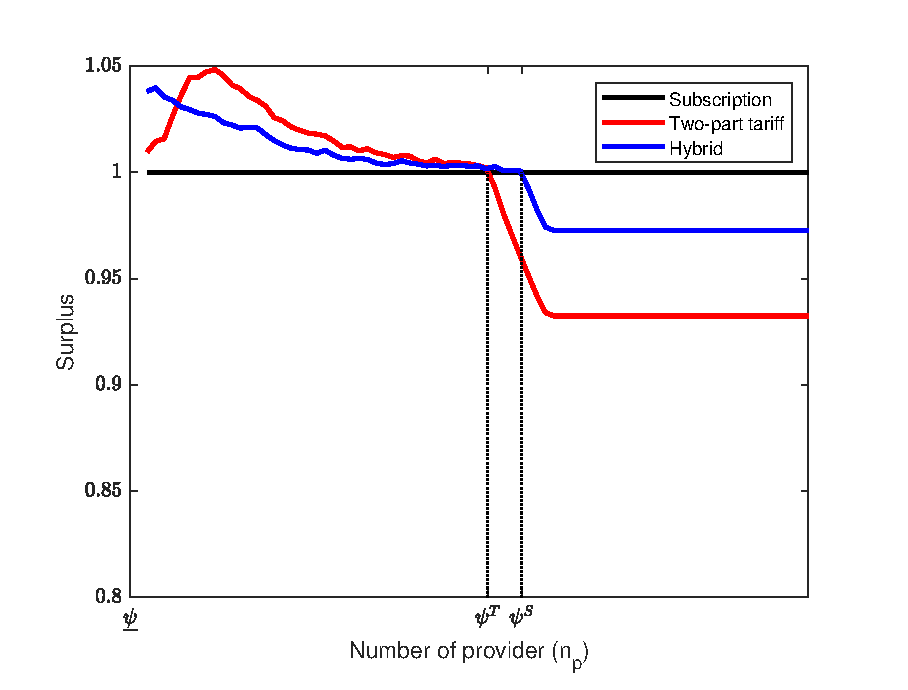
\includegraphics[width=5cm]{figure_3rd_final/prop_c_6_1.eps}}
    \textbf{\caption{Numerical Analysis for Utility Function I and Scenario \textit{ii}}}
\end{figure}
%- 아래의 pareto distribution에서 parameter가 달라질 때 효과와 연결\\
%- 용량이 큰 고객의 $b$가 큰 경우에, 이들에게는 i) first-best 인 부분에서 bandwidth에 비용을 지불받는 것의 merit이 줄어들어 subscription과 가까워짐 2) 마찬가지로 market-clearing에서도 bandwidth로부터 얻는 이익이 많이 없어져서 subscription과 가까워짐 -- c로 갈 수록 전체적으로 subscription과 가까워지는 모습(특히, hybrid)\\

%\textbf{Utility function II.}  When the bandwidth allowance is constant
\newpage
%\underline{\textit{Scenario i})} $(b_l, b_h) = (2, 2)$
\begin{figure}[ht!]
    \centering
    \subfigure[$Low:High = 9:1$]{\includegraphics[width=5cm]{figure_3rd_final/volume_c_1.eps}}
    \subfigure[$Low:High = 5:5$]{\includegraphics[width=5cm]{figure_3rd_final/volume_c_2.eps}}
    \subfigure[$Low:High = 1:9$]{\includegraphics[width=5cm]{figure_3rd_final/volume_c_3.eps}}
    \textbf{\caption{Numerical Analysis for Utility Function II and Scenario \textit{i}}}
\end{figure}

%\underline{\textit{Scenario ii})} $(b_l, b_h) = (2, 5)$
%%%%%%%%%%%%%%%%%%
\begin{figure}[ht!]
    \centering
    \subfigure[$Low:High = 9:1$]{\includegraphics[width=5cm]{figure_3rd_final/volume_c_4.eps}}
    \subfigure[$Low:High = 5:5$]{\includegraphics[width=5cm]{figure_3rd_final/volume_c_5.eps}}
    \subfigure[$Low:High = 1:9$]{\includegraphics[width=5cm]{figure_3rd_final/volume_c_6.eps}}
    \textbf{\caption{Numerical Analysis for Utility Function II and Scenario \textit{ii}}}
\end{figure}

\subsection{Hybrid Pricing and Profit Comparison}
In this numerical analysis, we compare a variety of $Hh$-type hybrid pricing schemes (i.e., $q>1$) with a two-part tariff and subscription-based pricing across different numbers of providers ($n_p$), redundancy rate ($\theta$) operating costs ($\xi$), and minimum download volumes ($\lambda_0$). Specifically, we consider the three following scenarios:

\begin{itemize}
    \item \textbf{Scenario 1: $(\theta, \xi, \lambda_0) = (2, 1.2, 2)$}
    \item \textbf{Scenario 2: $(\theta, \xi, \lambda_0) = (5, 1.2, 2)$}
    \item \textbf{Scenario 3: $(\theta, \xi, \lambda_0) = (2, 0.9, 1)$}
\end{itemize}

Note that we allow the number of providers ($n_p$) to change continuously within each scenario. Based on the parameter scenarios and the continuous $n_p$ region, we experiment with multiple values of free bandwidth allowance: 1 (or a two-part tariff), 1.05, 1.1., 2, 5, 10, 100, and $\infty$ (or subscription). In doing so, we fix $\alpha = 0.95$ and $n_r = 100$, and all parameter sets we consider here hold $\xi > \frac{3}{4}\alpha$.

\textbf{Figure C.8} shows the graphical results of our numerical analysis. On the left-hand side---i.e., \textbf{Figures C.8.}(a), (c), and (e), we present the absolute profit values by pricing scheme. We find that all these scenarios and $n_p$ regions show consistent patterns: the higher free bandwidth (i.e., higher $q$), the lower profit. As $q$ increases (from $q=1.05$ to $q=100$), the profit of hybrid pricing goes further away from that of the two-part tariff (line $T$) and approaches that of subscription-based pricing (line $S$).

Because the profit lines for the two-part tariff ($T$) and two small $q$'s ($q=1.05$ and $q=1.1$) overlap with each other on the profit plots, we zoom in on their relationships by plotting relative profits among these pricing schemes on the right-hand side---i.e., \textbf{Figures C.8.}(b), (d), and (f). Here, the vertical axis indicates the relative profits of hybrid pricing, which is each pricing scheme's profit divided by the two-part tariff's profit. We observe consistent patterns; that is, the higher $q$, the lower the relative profit.

% parameter sets:
% fixed : $\alpha = 0.95$, $n_r = 100$
% varied: $(\theta, \xi, \lambda_0) = (2, 1.2, 2)$, $(\theta, \xi, \lambda_0) = (5, 1.2, 2)$, $(\theta, \xi, \lambda_0) = (2, 0.9, 1)$
% Note., all parameter sets hold $\xi > \frac{3}{4}\alpha$.\\

\begin{figure}[ht!]
    \centering
    \subfigure[Profit (Scenario 1)]{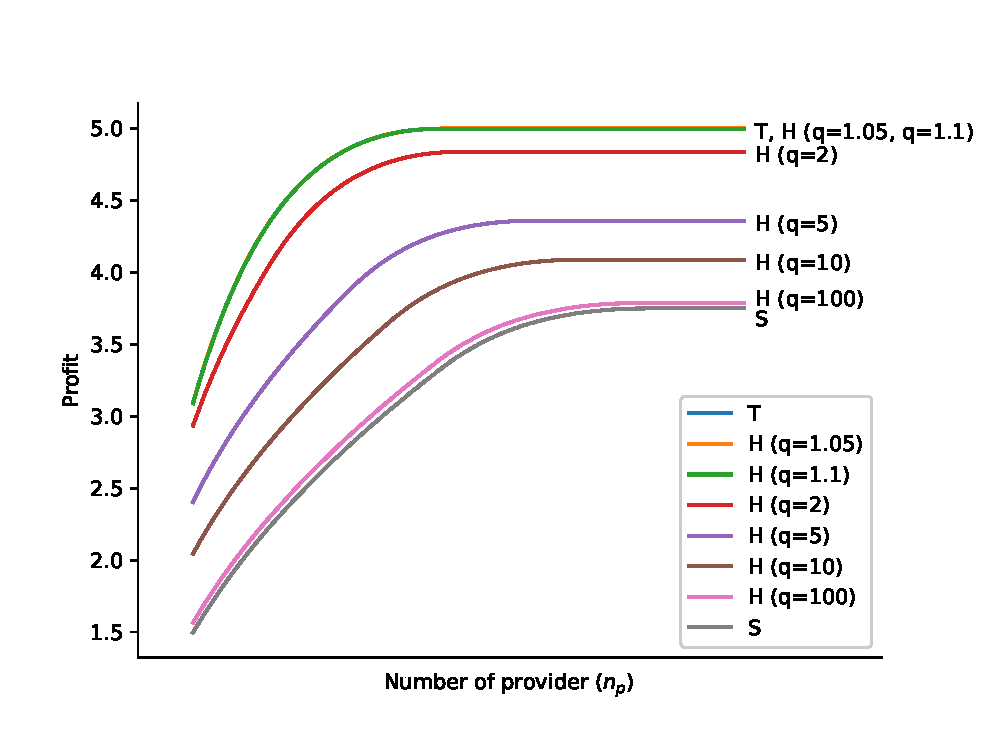
\includegraphics[width=7.5cm]{figure_3rd_final/p2pnum11.eps}}
    \subfigure[Relative profit (Scenario 1)]{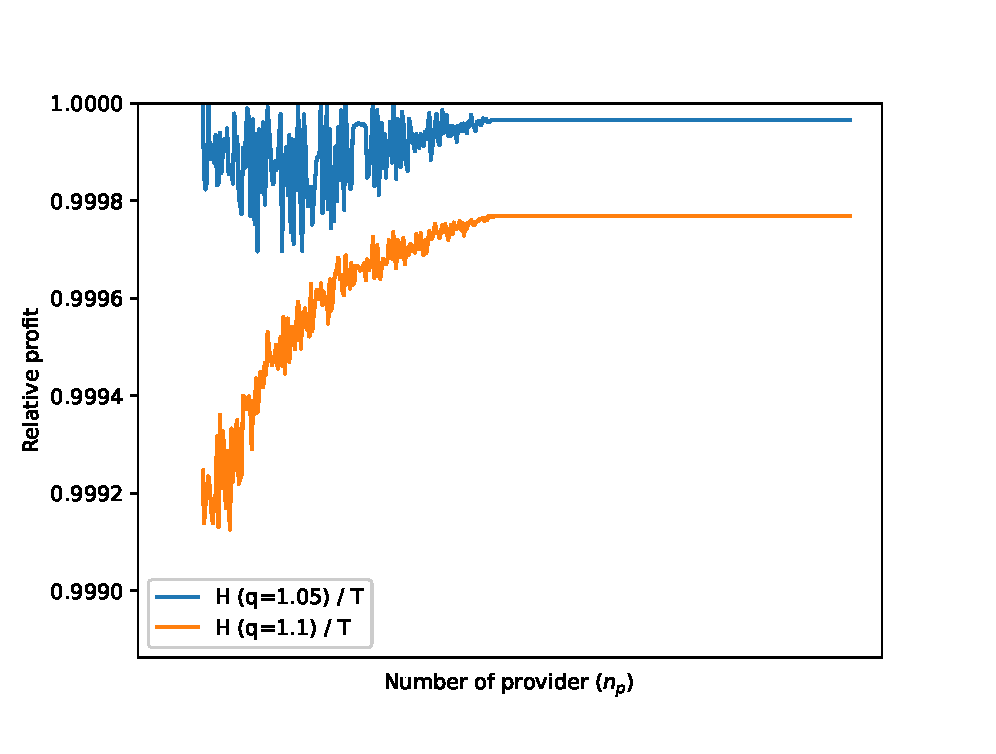
\includegraphics[width=7.5cm]{figure_3rd_final/p2pnum21.eps}}
    \subfigure[Profit (Scenario 2)]{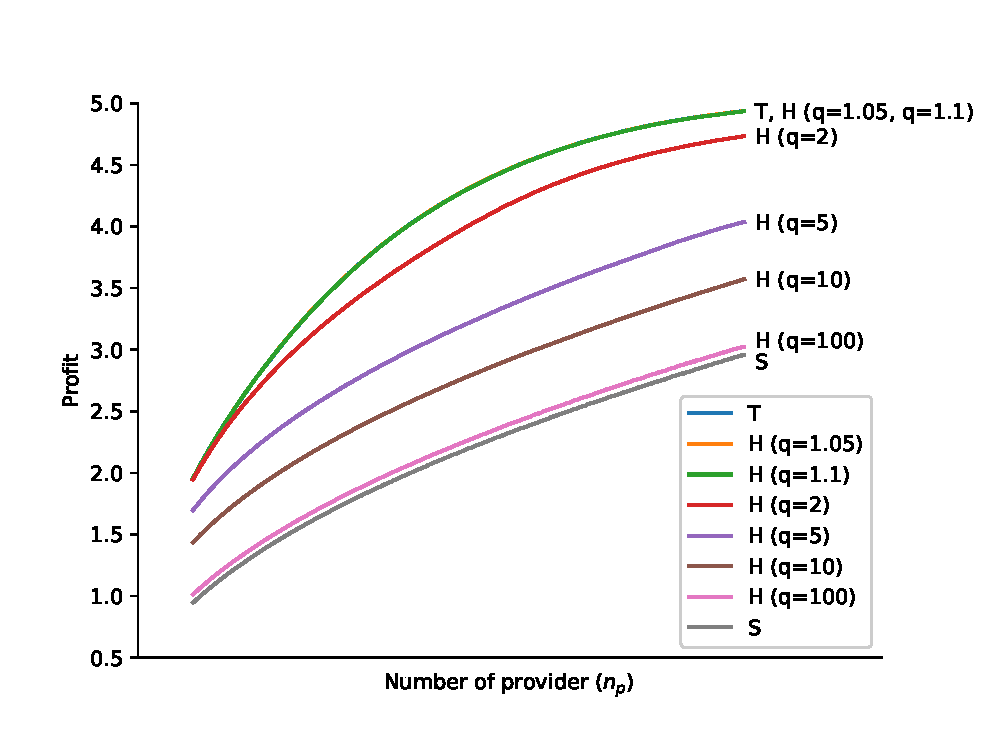
\includegraphics[width=7.5cm]{figure_3rd_final/p2pnum1a.eps}}
    \subfigure[Relative profit (Scenario 2)]{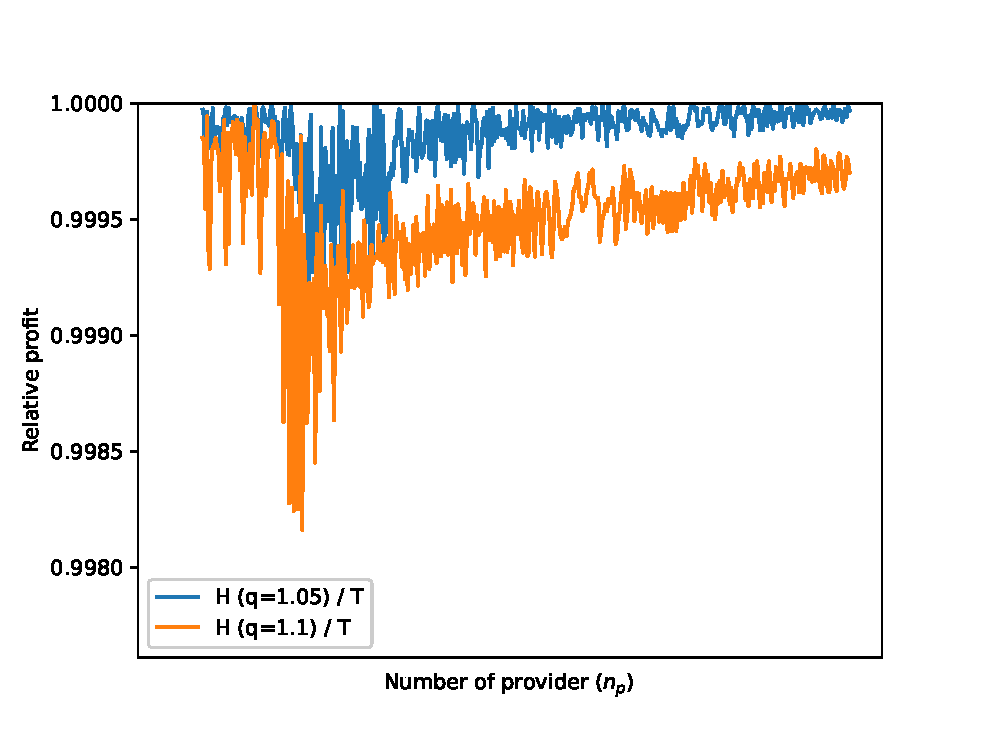
\includegraphics[width=7.5cm]{figure_3rd_final/p2pnum2a.eps}}
    \subfigure[Profit (Scenario 3)]{\includegraphics[width=7.5cm]{figure_3rd_final/p2pnum1b.eps}}
    \subfigure[Relative profit (Scenario 3)]{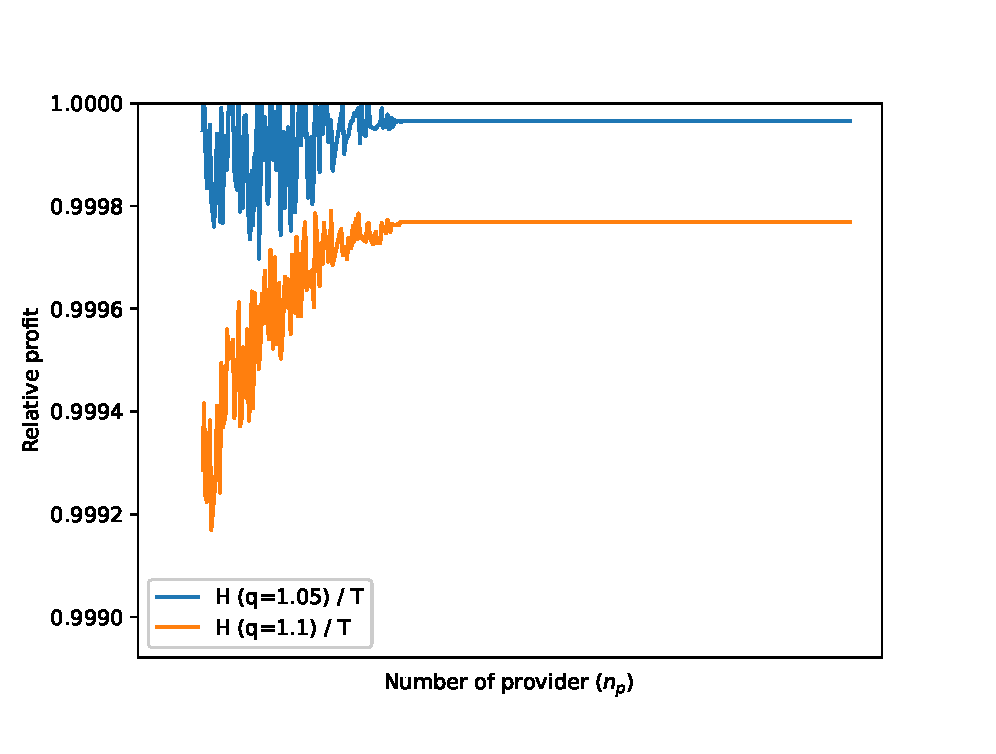
\includegraphics[width=7.5cm]{figure_3rd_final/p2pnum2b.eps}}
    \textbf{\caption{Numerical Analysis of Profit Comparison
}}
\end{figure}

\end{document}